\documentclass[type=doctor]{thuthesis}
% 选项:
%   type=[bachelor|master|doctor|postdoctor], % 必选
%   secret,                                   % 可选
%   pifootnote,                               % 可选(建议打开)
%   openany|openright,                        % 可选,基本不用
%   arial,                                    % 可选,基本不用
%   arialtoc,                                 % 可选,基本不用
%   arialtitle                                % 可选,基本不用

% 所有其它可能用到的包都统一放到这里了,可以根据自己的实际添加或者删除。
\usepackage{thuthesis}
\usepackage{tikz}
\usetikzlibrary{arrows.meta} 
\usepackage{tensor}
\usepackage{xspace}
\usepackage{alltt}
%\usepackage{pdflscape}
\usepackage{lscape} 
\usepackage[boxed]{algorithm2e}
\usepackage{mathpartir}
\usepackage{amssymb}
\usepackage{wasysym}
\usepackage{marvosym}
\usepackage{pifont}



%\usepackage{amsmath,amssymb,latexsym} 
%\usepackage{stmaryrd}

% 定义所有的图片文件在 figures 子目录下
\graphicspath{{figures/}}

% 可以在这里修改配置文件中的定义。导言区可以使用中文。
% \def\myname{薛瑞尼}

%%% calligraphic letters
\newcommand{\cA}{\mathcal{A}}
\newcommand{\cB}{\mathcal{B}}
\newcommand{\cC}{\mathcal{C}}
\newcommand{\cD}{\mathcal{D}}
\newcommand{\cE}{\mathcal{E}}
\newcommand{\cF}{\mathcal{F}}
\newcommand{\cG}{\mathcal{G}}
\newcommand{\cH}{\mathcal{H}}
\newcommand{\cI}{\mathcal{I}}
\newcommand{\cL}{\mathcal{L}}
\newcommand{\cM}{\mathcal{M}}
\newcommand{\cN}{\mathcal{N}}
\newcommand{\cO}{\mathcal{O}}
\newcommand{\cP}{\mathcal{P}}
\newcommand{\cR}{\mathcal{R}}
\newcommand{\cS}{\mathcal{S}}
\newcommand{\cT}{\mathcal{T}}
\newcommand{\cV}{\mathcal{V}}
\newcommand{\cX}{\mathcal{X}}
\newcommand{\cY}{\mathcal{Y}}

%%% brackets
\newcommand{\lb}{\langle}
\newcommand{\rb}{\rangle}

%%% arrows
\newcommand{\la}{\leftarrow}
\newcommand{\ra}{\rightarrow}
\newcommand{\da}{\downarrow}
\newcommand{\ua}{\uparrow}
\newcommand{\dive}{\uparrow\vspace{0.5mm}\uparrow}
\newcommand{\lra}{\leftrightarrow}
\newcommand{\lh}{\leftharpoons}
\newcommand{\rh}{\rightharpoons}
\newcommand{\rlh}{\rightleftharpoons}
\newcommand{\Lla}{\longleftarrow}
\newcommand{\Lra}{\longrightarrow}
\newcommand{\Llra}{\longleftrightarrow}
\newcommand{\Dla}{\Leftarrow}
\newcommand{\Dra}{\Rightarrow}
\newcommand{\Dda}{\Downarrow}
\newcommand{\Dua}{\Uparrow}
\newcommand{\Dlra}{\Leftrightarrow}
\newcommand{\Nla}{\not\rightarrow}
\newcommand{\Nra}{\not\leftarrow}
\newcommand{\raa}{\ra_{aliens}}
\newcommand{\rac}{\ra_{cap}}
\newcommand{\raA}{\ra_{A}}
\newcommand{\raC}{\ra_{C}}
%\newcommand{\nf}[1]{#1\!\!\downarrow}

\newcommand{\Var}[1]{\mathcal{V}ar({#1})}
\newcommand{\FVar}[1]{\mathcal{FV}ar({#1})}
\newcommand{\Pos}[1]{\mathcal{P}os({#1})}
\newcommand{\FPos}[1]{\mathcal{FP}os({#1})}
\newcommand{\VPos}[1]{\mathcal{VP}os({#1})}
\newcommand{\rootp}{\mbox {\footnotesize $\Lambda$}}
\newcommand{\Dom}[1]{\mathcal{D}om({#1})}
\newcommand{\TFX}{\cT(\cF,\cX)}
\newcommand{\GTF}{\cT(\cF)}
\newcommand{\Ran}[1]{{\cV\cR}an({#1})}

\renewcommand{\emptyset}{\varnothing}

%%% macros specifiques
\newcommand{\nat}{\mbox{$I\!\!N$}}
\newcommand{\vect}[1]{\overline{#1}}
%\newcommand{\interp}[1]{\mbox{$[\!\mid \!\! #1 \!\! \mid\!]$}}
\newcommand{\interp}[1]{\llbracket #1 \rrbracket}
%\newcommand{\Ft}{\mbox{$F_{\textit{T}}$}\xspace}
%\newcommand{\Fnt}{\mbox{$F_{\textit{NT}}$}\xspace}




%%% orders
% for labels
\newcommand{\ordl}{\gtordl}
\newcommand{\gtordl}{\rhd}
\newcommand{\geordl}{\unrhd}
\newcommand{\ltordl}{\lhd}
\newcommand{\leordl}{\unlhd}
% for positions
\newcommand{\gtordp}{>_{\cP}}
\newcommand{\geordp}{\ge_{\cP}}
\newcommand{\ltordp}{<_{\cP}}
\newcommand{\leordp}{\le_{\cP}}
\newcommand{\ordp}{\gtordp}
% for subsumption
\newcommand{\gtsubs}{\gtrdot}   %{{\scriptsize \bullet}{\hspace{-0.75mm}>}}
\newcommand{\gesubs}{\mathrel{\stackrel{\scriptscriptstyle\bullet}{}{\!\!\!\!\geq}}}
%\newcommand{\gesubs}{\mathrel{\cdot\!\!\!\geq}}
% for conversions
\newcommand{\po}{\mathrel{\succ\!\!\succ}}
\newcommand{\poeq}{\mathrel{\succeq\!\!\succeq}}
% others
\newcommand{\ordo}{\succ}
\newcommand{\rpo}{\succ_H}
\newcommand{\gerpo}{\succeq_H}
\newcommand{\rpomul}{\,(\rpo)_{mul}\,}
\newcommand{\gerpomul}{\,(\gerpo)_{mul}\,}



\newcommand{\cp}[1]{\cC\cP(#1)}
\newcommand{\pcp}[1]{\cP\cC\cP(#1)}
\newcommand{\hcp}[1]{\cH\cC\cP(#1)}

\newcommand{\lmm}[1]{\vect{#1}}
\newcommand{\mm}[1]{mm({#1})}

%\newcommand{\lll}[1]{ll(#1)}
\newcommand{\rll}[1]{rl(#1)}
\newcommand{\ml}[1]{\cL(#1)}

\newcommand{\fp}[1]{\mbox{\textsc{F}$_{\textsc p}$($#1$)}}
\newcommand{\vL}[1]{{\textsc{vl}}(#1)}
\newcommand{\vS}[1]{{\textsc{vs}}(#1)}
\newcommand{\vs}[1]{{\textsc{sh}}(#1)}
\newcommand{\hp}[1]{\cH p(#1)}
\newcommand{\hit}[1]{\cH t(#1)}
\newcommand{\IC}[1]{\cI\cC(#1)}
\newcommand{\lp}[1]{#1_{\mathit{peak}}}
\newcommand{\lc}[1]{#1_{\mathit{conv}}}
\newcommand{\lcl}[1]{#1_{\mathit{cliff}}} %added by jiaxiang
\newcommand{\lcp}[1]{#1_{\mathit{convp}}} %added by jiaxiang
\newcommand{\lcc}[1]{#1_{\mathit{convc}}} %added by jiaxiang

\newcommand{\equivp}[2]{~\equiv^{#1}_{#2}~}
\newcommand{\repl}{{\cR}epl}

%\newcommand{\RT}{R_{{\textsc{t}\xspace}}}
%\newcommand{\RNT}{R_{{\textsc{nt}\xspace}}}

%labelled rewriting
%Optional Args 1: position, 2:label, 3:rule or rule set, 4:substitution.
\newcommand{\lablrps}[4]{\mathop{\longrightarrow}^{#1,#2}_{#3,#4}}
\newcommand{\dlablrps}[4]{\displaystyle \lablrps{#1}{#2}{#3}{#4}}
\newcommand{\lablrpps}[4]{\mathop{\Longrightarrow}^{#1,#2}_{#3,#4}}
\newcommand{\dlablrpps}[4]{\displaystyle \lablrpps{#1}{#2}{#3}{#4}}

% rewriting
%% \newcommand{\lrps}[2]{{\mathop{\longrightarrow}^{#1}_{#2}}}
\newcommand{\lrps}[2]{\mathrel{\ra^{#1}_{#2}}} % new def
\newcommand{\llrps}[2]{~\lrps{#1}{#2}~}
\newcommand{\dlrps}[2]{\displaystyle \lrps{#1}{#2}}
\newcommand{\dllrps}[2]{\displaystyle \llrps{#1}{#2}}
%% \newcommand{\rlps}[2]{{^{~#1}_{#2}\!\!\mathop{\longleftarrow}}}
%%\newcommand{\rlps}[2]{\mathrel{\prescript{#1\!\!\;}{#2}{\!\!\;\la}}} % new def
%% \newcommand{\rlps}[2]{\mathrel{\myprescript{#1\!\!\;}{#2}{\!\!\;\la}}} % new def
\newcommand{\rlps}[2]{\mathrel{\!\tensor*[^{#1\!\!\;}_{#2}]{\!\!\;\la}{}}} % new def
\newcommand{\lrlps}[2]{~\rlps{#1}{#2}~}
\newcommand{\rlpsbis}[2]{\mathop{\longleftarrow}^{\,#1}_{#2}}
\newcommand{\drlps}[2]{{\displaystyle \rlpsbis{#1}{#2}}}
\newcommand{\dlrlps}[2]{~\drlps{#1}{#2}~}
\newcommand{\Lrps}[2]{\mathrel{\Rightarrow^{#1}_{#2}}} % new def
\newcommand{\Rlps}[2]{\mathrel{\prescript{#1\!\!\;}{#2}{\!\!\;\Leftarrow}}} % new def

%\newcommand{\DLrps}[2]{\mathop{\Longrightarrow}^{#1}_{#2}}
%\newcommand{\TLrps}[2]{\mathop{\Longrightarrow\!\!\succ}^{#1}_{#2}}

% parallel rewriting
%\newcommand{\llrpps}[2]{~\Lrps{#1}{#2}~}
%\newcommand{\Rlps}[2]{\mathop{\Longleftarrow}^{#1}_{#2}}
%\newcommand{\lrlpps}[2]{~\Rlps{#1}{#2~}}

%% symmetric closures
\newcommand{\eqps}[2]{\mathrel{\lra^{#1}_{#2}}} % new def
\makeatletter
\newcommand{\shorteq}{%
  \settowidth{\@tempdima}{-}% Width of hyphen
  \resizebox{\@tempdima}{\height}{=}%
}
\makeatother
%% \newcommand{\eqpseq}[2]{{\mathop{\:\;{\tiny =}\:\!\!\!\!\!\!\!\!\!\!\!\longleftrightarrow}^{#1}_{#2}}}
\newcommand{\eqpseq}[2]{\mathrel{\mathrel{\lra\!\!\!\!\!\!\!\:\shorteq\,\,}^{#1}_{#2}}} % new def 
\newcommand{\deqpseq}[2]{\displaystyle \eqpseq{#1}{#2}}

%% \newcommand{\conv}[2]
%%            {{\mathop{\la\!\!\!\!\!\longleftrightarrow\!\!\!\!\!\ra}^{#1}_{#2}}}
\newcommand{\conv}[2]{\mathrel{\la\!\!\!\!\!\lra\!\!\!\!\!\ra^{#1}_{#2}}} % new def
\newcommand{\lconv}[2]{~\conv{#1}{#2}~}
\newcommand{\dconv}[2]{\displaystyle \conv{#1}{#2}}
\newcommand{\dlconv}[2]{~\dconv{#1}{#2}~}
%\newcommand{\conv}[1]{\displaystyle \convv{#1}}


%% reflexive closures
%% \newcommand{\lrpseq}[2]{{\mathop{\longrightarrow\!\!\!\!\!\!\!{\tiny =}}^{#1}_{#2}}}
\newcommand{\lrpseq}[2]{\mathrel{\mathrel{\ra\!\!\!\!\!\!\:\shorteq\,}^{#1}_{#2}}} % new def
\newcommand{\llrpseq}[2]{~\lrpseq{#1}{#2}~}
\newcommand{\dlrpseq}[2]{\displaystyle \lrpseq{#1}{#2}}
\newcommand{\dllrpseq}[2]{\displaystyle \llrpseq{#1}{#2}}
%% \newcommand{\rlpseq}[2]{{~^{~#1}_{#2}\mathop{\!{\tiny =}\!\!\!\!\!\!\!\longleftarrow}}}
\newcommand{\rlpseq}[2]{\mathrel{\prescript{#1\!\!\;}{#2}{\;\!\shorteq\!\!\!\!\!\!\:\la}}} % new def
\newcommand{\lrlpseq}[2]{~\rlpseq{#1}{#2}~}
\newcommand{\rlpseqis}[2]{\mathop{{\tiny =}\!\!\!\!\!\!\!\longleftarrow}^{#1}_{#2}}
\newcommand{\drlpseq}[2]{\,{\displaystyle \rlpseqis{#1}{#2}}}
\newcommand{\dlrlpseq}[2]{~\drlpseq{#1}{#2}~}
%\newcommand{\lrppseq}[1]{\mathop{\Longrightarrow\!\!\!\!\!\!\!{\tiny =}}^{#1}}
%\newcommand{\rlppseq}[1]{\mathop{{\tiny =}\!\!\!\!\!\!\!\Longleftarrow}^{#1}}


%% derivations
%% \newcommand{\lrder}[2]{{\mathop{\longrightarrow\!\!\!\!\!\ra}^{#1}_{#2}}}
\newcommand{\lrder}[2]{\mathrel{\ra\!\!\!\!\!\ra^{#1}_{#2}}} % new def
\newcommand{\llrder}[2]{~\lrder{#1}{#2}~}
\newcommand{\dlrder}[2]{\displaystyle \lrder{#1}{#2}}
\newcommand{\dllrder}[2]{~\dlrder{#1}{#2}~}
%% \newcommand{\rlder}[2]{{~^{~#1}_{#2}\!\!\mathop{\la\!\!\!\!\!\longleftarrow}}}
\newcommand{\rlder}[2]{\mathrel{\prescript{#1\!\!\;}{#2}{\!\!\;\la\!\!\!\!\!\la}}} % new def
\newcommand{\lrlder}[2]{~\rlder{#1}{#2}~}
\newcommand{\rlderis}[2]{\mathop{\la\!\!\!\!\!\longleftarrow}^{~#1}_{#2}}
\newcommand{\drlder}[2]{{\displaystyle \rlderis{#1}{#2}}}
\newcommand{\dlrlder}[2]{~\drlder{#1}{#2}~}

\newcommand{\ordt}{\mbox{$\succ\!\!\succ$}}
\newcommand{\geordt}{\mbox{$\succeq\!\!\succeq$}}

%% others
\newcommand{\LrpsD}{\Longrightarrow_\cD}
\newcommand{\RlpsD}{_\cD\!\!\Longleftarrow}



\newcommand{\hide}[1]{\ignorespaces}
\newcommand{\todo}[1]{\textbf{TODO: } #1}
\renewcommand{\algorithmcfname}{算法}

\newcommand{\zero}{\operatorname{\mathsf{zero}}}
\newcommand{\s}{\operatorname{\mathsf{s}}}
\newcommand{\add}{\operatorname{\mathsf{add}}}
\newcommand{\lessthan}{\operatorname{\mathsf{lessthan}}}
\newcommand{\true}{\operatorname{\mathsf{true}}}
\newcommand{\false}{\operatorname{\mathsf{false}}}
\newcommand{\mynot}{\operatorname{\mathsf{not}}}
\newcommand{\farmer}{\operatorname{\mathsf{farmer}}}
\newcommand{\wolf}{\operatorname{\mathsf{wolf}}}
\newcommand{\lamb}{\operatorname{\mathsf{lamb}}}
\newcommand{\grass}{\operatorname{\mathsf{grass}}}
\newcommand{\lhs}{\operatorname{\mathsf{left}}}
\newcommand{\rhs}{\operatorname{\mathsf{right}}}
\newcommand{\change}{\operatorname{\mathsf{change}}}
\newcommand{\comp}{\operatorname{\mathsf{::}}}
\renewcommand{\clock}{\operatorname{\mathsf{clock}}}
\newcommand{\broken}{\operatorname{\mathsf{broken}}}
\newcommand{\myempty}{\operatorname{\mathsf{empty}}}

\newcommand{\defeq}{\ensuremath{\stackrel{\text{\tiny def}}{=}}}
\newcommand{\nf}[2]{{#1}\!\da_{#2}\xspace}
\newcommand{\RE}{\cR_{\cE}}
\newcommand{\SE}{\cS_{\cE}}
\newcommand{\RSE}{\cR_{\cS\cE}}
\newcommand{\VP}{\cV_{\cP}}
\newcommand{\Vsym}{\cV_{sym}}
\newcommand{\pta}{\hookrightarrow}
\newcommand{\ty}{\texttt{ty}}
\newcommand{\transto}{\rightsquigarrow}

\newcommand{\allsup}{\ding{51}}
\newcommand{\halfsup}{\CheckedBox}
\newcommand{\nonsup}{\ding{55}}

\newcommand\TTT{%
 \textsf{T\kern-0.2em\raisebox{-0.3em}T\kern-0.2emT\kern-0.2em\raisebox{-0.3em}2}%
}

\newcommand{\CTerm}{{Ceagle-\textsc{Term}}}

\begin{document}

%%% 封面部分
\frontmatter
\thusetup{
  %******************************
  % 注意:
  %   1. 配置里面不要出现空行
  %   2. 不需要的配置信息可以删除
  %******************************
  %
  %=====
  % 秘级
  %=====
  secretlevel={秘密},
  secretyear={10},
  %
  %=========
  % 中文信息
  %=========
  ctitle={基于重写理论的\\嵌入式系统建模与验证},
  cdegree={工学博士},
  cdepartment={计算机科学与技术系},
  cmajor={计算机科学与技术},
  cauthor={刘嘉祥},
  csupervisor={顾 明教授},
  cassosupervisor={孙家广教授}, % 副指导老师
  % ccosupervisor={某某某教授}, % 联合指导老师
  % 日期自动使用当前时间,若需指定按如下方式修改:
  % cdate={超新星纪元},
  %
  % 博士后专有部分
  cfirstdiscipline={计算机科学与技术},
  cseconddiscipline={系统结构},
  postdoctordate={2009年7月——2011年7月},
  id={编号}, % 可以留空: id={},
  udc={UDC}, % 可以留空
  catalognumber={分类号}, % 可以留空
  %
  %=========
  % 英文信息
  %=========
  etitle={Rewriting-Based Modeling and Verification of Embedded Systems},
  % 这块比较复杂,需要分情况讨论:
  % 1. 学术型硕士
  %    edegree:必须为Master of Arts或Master of Science(注意大小写)
  %             “哲学、文学、历史学、法学、教育学、艺术学门类,公共管理学科
  %              填写Master of Arts,其它填写Master of Science”
  %    emajor:“获得一级学科授权的学科填写一级学科名称,其它填写二级学科名称”
  % 2. 专业型硕士
  %    edegree:“填写专业学位英文名称全称”
  %    emajor:“工程硕士填写工程领域,其它专业学位不填写此项”
  % 3. 学术型博士
  %    edegree:Doctor of Philosophy(注意大小写)
  %    emajor:“获得一级学科授权的学科填写一级学科名称,其它填写二级学科名称”
  % 4. 专业型博士
  %    edegree:“填写专业学位英文名称全称”
  %    emajor:不填写此项
  edegree={Doctor of Philosophy}, 
  emajor={Computer Science and Technology},
  eauthor={Liu Jiaxiang},
  esupervisor={Professor Gu Ming},
  eassosupervisor={Professor Sun Jiaguang},
  % 日期自动生成,若需指定按如下方式修改:
  % edate={December, 2005}
  %
  % 关键词用“英文逗号”分割
  ckeywords={形式化方法, 嵌入式系统, 规范化条件重写模型, 建模, 验证},
  ekeywords={formal methods, embedded systems, normalization conditional rewrite sytems, modeling, verification}
}

% 定义中英文摘要和关键字
\begin{cabstract}
随着嵌入式系统与现代社会生产、生活越来越深度的结合,其可靠性和安全性也变得与人们的生命财产安全息息相关,利用形式化方法对嵌入式系统进行验证以保证其正确性的需求日益迫切。形式化模型作为形式化验证方法的核心,是影响它在嵌入式系统中进行应用的关键因素。现代嵌入式系统中多线程技术的应用以及系统与外界环境复杂的交互,对形式化模型的建模能力和验证能力都提出了更高的要求。

重写模型适用于对多线程行为进行建模,且支持模型检测、定理证明等多种形式化验证技术,近年来受到形式化验证领域的关注。将重写模型应用于嵌入式系统的实际验证项目中,目前面临两个问题:(1) 如何在行为具有不确定性的重写模型中描述嵌入式软件的顺序行为;(2) 如何提高易用性,降低重写模型的建模成本。围绕这两个问题,本文提出了一个形式化模型——规范化条件重写模型,且基于该模型设计开发了一套针对嵌入式系统的建模方法以及一个针对 C 语言程序的终止性验证工具 \CTerm:

\begin{enumerate}
\item
针对重写模型对顺序行为表达能力的局限性,本文提出能够支持确定性行为描述的规范化条件重写模型。规范化条件重写模型支持自定义数据类型,具备描述状态等价、条件控制的表达能力,也能够对以硬件并发行为为代表的不确定性行为、以及以软件顺序行为为代表的确定性行为进行描述和语义区分。
\item
针对模型易用性问题,以建模方法论为切入点,本文基于规范化条件重写模型,提出一套对嵌入式系统结构层次性、行为异构性、结构动态性和实时性等特征的建模方法,旨在对建模过程进行指导。基于语义映射的方式,本文对该建模框架予以实现,并通过对两个真实嵌入式系统进行应用,验证了该方法在嵌入式系统中实际应用的可行性。
\item 
针对模型易用性问题,以嵌入式系统软件的自动建模为另一切入点,本文开发了一套基于规范化条件重写模型的 C 程序终止性自动验证工具 \CTerm,为系统的完全正确性提供了必要的工具支持。
\end{enumerate}

作为本文的应用案例之一,机车优化控制系统目前运行稳定,并在沈阳铁路局通过了实车运用考核;而经过本文建模验证的速率单调调度系统目前在某工业级航天控制器中在线运行。
\end{cabstract}

% 如果习惯关键字跟在摘要文字后面,可以用直接命令来设置,如下:
% \ckeywords{\TeX, \LaTeX, CJK, 模板, 论文}

\begin{eabstract}

Embedded systems are increasingly used in the modern society, becoming 
embedded in our lives. Due to the importance of their reliability and safety, 
formal methods for verifying the correctness of embedded systems are in great demand. As the heart of formal verification methods, formal models are the key to their application on embedded systems. Multithreading techniques are deployed in the modern systems, and there exists complicated interaction between embedded systems and their environment. Both will raise new challenges to the formal models about their abilities to model and verify.

Recently, rewrite systems have won attention for formal verification, given the facts that they are suitable for modeling the behaviors of multithreads and they support multiple verification techniques such as model checking and theorem proving. To apply rewrite systems on realistic verification projects for embedded systems, we need to answer two questions: (1) How do we capture sequential behaviors via rewrite systems inheriting non-determinism? (2) How do we enhance the usability of rewrite systems to ease the modeling process? To answer these questions, this dissertation introduces a new formal model named \emph{normalization conditional rewrite systems}. Based on the new model, we develop a methodology for modeling embedded systems and a termination prover \CTerm for C programs:

\begin{enumerate}
\item Aimed at the limitation of rewrite systems for expressing sequential behaviors, this dissertation introduces normalization conditional rewrite systems, which are able to describe deterministic behaviors. Normalization conditional rewrite systems support user-defined data types and the expressivity for state equivalence and conditional branching. They can also model and distinguish the semantics of non-deterministic behaviors, such as those concurrently in hardware, and of deterministic behaviors, such as those sequentially in software. 
\item Aimed at the usability of the model, focusing on modeling methodologies, this dissertation proposes a methodology which captures the hierarchy, the heterogeneous behaviors, the dynamic structures and the real-timeness of embedded systems. We implement the methodology based on semantics mapping. Then we demonstrate its feasibility for application, by applying it on two realistic embedded systems. 
\item Aimed at the usability of the model, focusing on the automatic construction of models of embedded software, this dissertation develops an automatic termination prover \CTerm for C programs based on normalization conditional rewrite systems. The tool provides possibility to prove total correctness of systems.  
\end{enumerate}

As one of the case studies, the Train Optimized Control System is currently in smooth operation, and passes the on-board test by Shenyang Railway Administration; the formally verified Rate-Monotonic Scheduling System by this dissertation has been serving in some industrial avionic control system.
\end{eabstract}

% \ekeywords{\TeX, \LaTeX, CJK, template, thesis}

% 如果使用授权说明扫描页,将可选参数中指定为扫描得到的 PDF 文件名,例如:
% \makecover[scan-auth.pdf]
\makecover  

%% 目录
\tableofcontents

%% 符号对照表
\begin{denotation}[3cm]
\item[FSM] 有限状态机 (Finite State Machine)
\item[HCFSM] 层次化并发有限状态机 (Hierarchical Concurrent FSM)
\item[CPN] 着色 Petri 网 (Colored Petri Net)
\item[LTL] 线性时序逻辑 (Linear Temporal Logic)
\item[CIC] 归纳构造演算 (Calculus of Inductive Constructions)
\item[HOL] 高阶逻辑 (Higher-Order Logic)
\item[RTL] 寄存器转换语言 (Register Transfer Language)
\item[$\cF$] 词汇表
\item[$\cX$] 可数的变量符号集合
\item[$\TFX$] 项表达式集合
\item[$\cR$] 重写模型
\item[$\cE$] 等价模型
\item[$\cR_{\cE}$] 模重写模型
\item[$\RSE$] 规范化条件重写模型
\item[$\mathcal{R^L}$] 重写逻辑模型
\item[RMS] 速率单调调度 (Rate-Monotonic Scheduling)
\item[PC] 程序计数器 (Program Counter)
\item[CTL] 分支时态逻辑 (Computation Tree Logic)
\item[$\cR_{\cI}$] 整数重写模型
\item[TPDB] 终止性问题数据库 (Termination Problems Data Base)
\item[DSL] 领域特定语言 (Domain Specific Language)
\end{denotation}




%%% 正文部分
\mainmatter
\chapter{绪论}
\label{cha:intro}

\section{研究背景}

\emph{嵌入式系统}~\cite{heath2002embedded} 最早出现在六十年代,其产生是为了减少搭载系统的体积重量以及降低成本。作为计算资源的成本高昂的计算机逐步被成本相对低廉的微处理器系统替换,导致设备不仅变得小型化、低价格,同时处理能力以及功能也不断提高。这些变化使得七八十年代时期,民用电子、消费类电子等行业得到了快速发展并大规模兴起。从工业 2.0 时代开始的自动化、电力驱动的大规模工业生产中,早期的嵌入式系统开始大量投入使用。到现在的工业3.0时代以及2013年德国提出的工业4.0,以信息化、智能化、自动化、网络化作为核心,数字化产品以及产品生产制造过程,其全生命周期都将依赖于电子信息而产生的新工业模式。在这中间,嵌入式系统的不断强大将为工业的进程提供技术支撑,以加快工业 4.0 在全领域的普及。

最早,不同的嵌入式系统承载不同功能,其设计是为特定系统、特定任务而定制的,大多数嵌入式系统都是功能单一的系统。在发展过程中,嵌入式系统的处理单元逐渐变得强大(如现在的 ARM、PowerPC、MIPS 等),外围设备、硬件资源越来越丰富,使其可以承担更多复杂的处理任务,并具有了通用性、架构可移植的特点。在嵌入式系统硬件能力提升的基础上,除了为硬件系统开发固件外,Linux、MS-DOS,以及专为嵌入式系统开发的实时操作系统 VxWorks 等操作系统的加入,可以完成系统设备的协调调度、资源监管等任务,并且使得开发运行针对应用需求的用户控制界面和具有更多功能的应用软件成为可能。 

除消费类电子产品外,嵌入式系统在民用、军用大型设备中的作用同样重要。在航空领域中,民用航空飞机的机载电子设备功能越发强大,系统架构也越发复杂。飞行控制系统、导航系统、通信系统、雷达系统、环境控制系统,以及各终端传感器系统都搭载了嵌入式系统来对其进行控制,并完成计算、存储、传输等以支持飞控、通信、导航等高级任务。其中系统异步、并发、调度、实时等问题引起的不确定性都是影响系统正常工作、影响飞行安全的重要因素。安全性是民用飞机的重要属性,系统安全性的设计、验证以及管理贯穿飞行器整个生命周期。有 ARP4754~\cite{ARP4754A}、ARP4761~\cite{ARP4761} 来指导飞行器系统的安全性设计,以及 DO-178C、DO-254 来指导符合安全性等级的软件、硬件设计。其中嵌入式系统的硬件要满足安全性设计中对应的可靠性需求,而固件及软件系统则要满足对应的软件验证需求。如飞控系统的安全性等级为 A 级,其涉及的嵌入式系统硬件设备要满足安全性保障等级为 A 的设计、测试、验证流程;对于其系统软件,则要求其设计及验证过程中必须使用严格的\emph{形式化方法} 对其安全等级进行保障。其它安全攸关的系统,如轨道运输、海洋运输都有相应的安全性保障需求。嵌入式系统硬件设计验证方法早已比较成熟,但是软件的形式化设计验证方法相对于硬件起步较晚。随着嵌入式系统软件发展的加快,针对嵌入式系统软件的形式化设计与验证存在迫切需求。在嵌入式系统的设计与开发过程中,硬件与软件往往是难以分开单独设计的,因为其软件及固件开发的专用性,互相影响程度很深。所以一种基于形式化方法的、可以同时对硬件及软件系统进行验证的方法亟待研究。

形式化建模与验证方法的基本流程如图~\ref{f:modeling-and-verification} 所示。建模人员需要先对目标系统进行手工或自动建模,得到系统的行为模型。针对系统的行为模型,验证人员再根据其关心的系统属性,利用相应的验证技术,如\emph{模型检测}~\cite{clarke1999model}(model checking)、\emph{定理证明}~\cite{DBLP:books/daglib/0070484}(theorem proving)等,及其相应的工具对系统模型进行形式化验证,从而得到针对属性的验证结果。根据验证结果,开发人员可以对目标系统进行修改或调整。在整个流程中,形式化的系统模型作为连接建模过程和验证过程的桥梁,对建模的难易程度、精确程度及验证的效果都起着至关重要的作用,是整个形式化建模验证方法的基础。

\begin{figure}[ht]
\centering
\includegraphics[width=\textwidth]{modeling-and-verification.jpg}
\caption{形式化建模与验证基本流程}
\label{f:modeling-and-verification}
\end{figure}

在种类繁多的嵌入式系统中,存在一类系统,它们与环境存在频繁的交互:它们通过输入设备(如传感器等)从环境接收周期性或非周期性的输入,系统对这些输入进行处理,然后通过输出设备(如执行器等)将处理结果反馈到环境中。这类系统被称作\emph{反应式系统}~\cite{DBLP:conf/iccd/Koopman96,DBLP:books/daglib/0010292}(reactive system)。大部分嵌入式系统都是反应式的:小到我们身边的消费类电子产品(如智能穿戴设备),大到交通运输系统(如第~\ref{s:TO} 小节讨论的机车控制系统)。由于反应式系统的输入不是单一的数值或事件,而是一个可能无穷的输入序列,这一显著特征从两个方面对形式化建模验证所使用的形式化模型提出了要求。
\begin{enumerate}
\item 
表达能力,即建模能力。随着现代嵌入式系统处理单元计算能力的提高,在硬件条件允许的情况下,多线程技术越来越多地被应用到反应式系统中~\cite{DBLP:conf/codes/GerndtE97,DBLP:journals/sigsoft/White11,DBLP:journals/tc/LiH12}。这一方面给系统引入了更多的并发性,要求形式化模型可以对并发行为进行描述;另一方面也要求形式化模型可以对线程的创建、释放等行为进行描述。出于对可组合性和层次化的考虑,线程一般被看作系统中的组件进行建模,于是线程的动态创建与释放行为要求形式化模型具有对系统结构动态变化的描述能力。
\item
验证能力。无穷的输入序列以及多线程带来的并发性使传统的模型检测技术可能面临状态空间爆炸的问题~\cite{DBLP:conf/ac/Valmari96}。因此,对反应式系统的形式化验证要求所使用的模型支持能解决状态空间爆炸的形式化验证技术,如定理证明。
\end{enumerate}

在下一小节中,我们将从上述两个方面对主流建模方法及形式化模型进行介绍和对比。

\section{研究现状}

嵌入式系统的建模方法不胜枚举,根据其描述对象的不同,可以建立架构模型、状态模型、数据模型等。它们分别以不同角度去描述嵌入式系统,用仿真、测试、形式化验证等方法保证系统的正确性、有效性、可靠性等多方面重要属性,特别是对安全攸关系统的设计、验证与运行提供有力支持。如上一节提到,嵌入式系统在众多安全攸关系统(如航空航天飞行器、铁路、核电站、医疗、保密系统等)中扮演着重要的角色。自 1990 年起,已有多份统计以研究报告与论文的形式指出形式化方法在工业领域中所取得的突出成果。2009 年英国约克大学的 Jim Woodcock 统计得到\cite{DBLP:journals/csur/WoodcockLBF09}:在工业应用中,对比只依赖于测试验证的工程开发,基于形式化建模与验证的工程项目有 92\% 得到了产品品质的提升,体现在更少的故障、正确性的提升、设计能力提升等多方面。

在这些形式化方法中,有些用抽象的形式化规约(specification)避免模型中的二义性,从而保证设计质量,如VDM~\cite{DBLP:conf/fm/1978}、Z~\cite{DBLP:books/daglib/0067866} 等。有些用状态模型描述系统行为特性,模型本身能够采用静态分析与模型执行来进行验证,如Petri网~\cite{murata1989}、自动机~\cite{DBLP:books/aw/HopcroftU79} 等。 

\emph{有限状态机}~\cite{minsky1967computation}(FSM)是面向系统状态最基本的模型,被控制系统广泛地应用。但对于功能、架构复杂的嵌入式系统,有限状态机缺乏对其并发性、实时性等方面的支持。所以有限状态机有多种扩展形式:支持并发性的\emph{层次化并发有限状态机}~\cite{DBLP:journals/scp/Harel87}(Hierarchical Concurrent FSM,HCFSM)以及支持时间的\emph{时间自动机}~\cite{DBLP:journals/tcs/AlurD94,DBLP:conf/cav/Alur99}(timed automata)。HCFSM可将一个状态组视为一个状态,状态组之间通过全局变量进行通信,可以用于描述多组件的、并发的控制系统。时间自动机作为有限状态机的另一个变种,增加对状态转移过程中时间因素的描述,变迁上标记的是该状态转移发生的时间约束,从而可以满足对实时系统时间分析的需求。然而,自动机及其扩展模型的模型结构是静态的,因此无法对系统结构的动态变化进行表达。

\textsc{Uppaal2k}~\cite{larsen1999uppaal2k},作为 \textsc{Uppaal}~\cite{DBLP:journals/sttt/LarsenPY97} 的后继工具,提供了对时间系统的建模、仿真以及验证功能,适用于对具有共享变量、通道通信的系统进行描述。\textsc{Uppaal2k} 支持对时间自动机图形化的建模、动态仿真以及模型检测等功能,可以进行有界活性检测、死锁检测、验证使用TCTL~\cite{DBLP:journals/logcom/BouchenebGR09}(Timed Computation Tree Logic)表达式描述的多种性质,不支持定理证明技术。

\emph{Petri 网}~\cite{murata1989} 的研究与应用相当广泛。由于对异步并发系统描述上的优势,Petri 网在实时系统、协议验证、硬件设计、制造过程、商业管理等众多领域中均发挥了作用~\cite{DBLP:journals/isci/KheldounBI17,DBLP:journals/jwe/XuPW17,DBLP:journals/tmc/ZhangAYM16,DBLP:conf/ACISicis/SalahBK15}。在实时嵌入式系统的应用中,Petri 网为描述待验证系统的异步、并发性、不确定性等多种特性提供了有效工具。虽然 Petri 网的网络结构是静态的,即它的三要素——库所、变迁以及有向弧不会发生改变,但由于 Petri 网的令牌(token)数量动态可变,且 Petri 网的状态由令牌分布决定,因此它可用于描述对象系统的结构变化。为了扩展标准 Petri 网的适应性,Petri 网衍生出多种变种,如着色 Petri 网~\cite{DBLP:series/eatcs/Jensen97}(Colored Petri Net,CPN)、对象 Petri 网~\cite{DBLP:conf/apn/Lakos95}(object Petri net)、混合 Petri 网~\cite{david2010discrete}(hybrid Petri net),
\hide{随机Petri网(stochastic Petri net),}
以及多种时间相关的 Petri 网,如 Time Petri Net~\cite{DBLP:journals/tse/BerthomieuD91}(TPN)、Timed Petri Net~\cite{DBLP:conf/isca/Zuberek80}(TdPN)、Timing Constraint Petri Net~\cite{DBLP:journals/tse/TsaiYC95}(TCPN),以适用于不同的应用需求。

\hide{
在以嵌入式实时系统为验证对象时,时间是最重要的因素之一,时间自动机以及各类时间 Petri 网均可在一定程度上满足描述以时间为关键因素的实时系统。根据描述对象的需求,将时间因素加入Petri网三个要素——库所、变迁以及有向弧上,扩展成为各种时间Petri网。这些时间Petri网虽然在描述时间约束上有不同的设计,但由于其不脱离标准Petri 网的形式化语法语义,基本可以实现相互之间的转化。TdPN以在变迁上的变迁时刻与延迟时间来表示该变迁转换时允许的最迟时间,即在规定阈值内到位的令牌仅可供该变迁使用。区别于TdPN,TPN所描述的系统不但要满足变迁上相应的时间延迟上限,而且需要满足变迁发生前所花费的最小时间,将变迁发生时间看作一个时间区间,以便更精确地对系统的运行时间进行分析与评估。由于其特点,TdPN与TPN都对并发系统具有一定的分析评估能力。而TCPN在库所与变迁上均可以增加时间约束,以表示触发过程的时间。与TdPN以及TPN不同,TCPN采用弱触发规则,即不满足时间约束时,由调度决策决定是否触发该变迁。因此,TCPN可以更准确地描述系统的执行过程。
}

在工具方面,一共有多达40多种工具提供了对时间相关的 Petri 网的支持。TINA~\cite{DBLP:conf/qest/BerthomieuV06}(TIme petri Net Analyzer)是其中应用最广泛的一种,可以对 TPN 和 TdPN 进行\emph{线性时序逻辑}~\cite{DBLP:conf/banff/Vardi95}(Linear Temporal Logic,LTL)性质验证、可达性验证等。Romeo~\cite{DBLP:conf/cav/GardeyLMR05} 是支持 TPN 验证的工具,并且预定义了多种从 TPN 到时间自动机的转换方法。这些工具基本都支持 Petri 网的建模、仿真及多种验证技术。

对于前面提到的时间自动机以及几种时间 Petri 网,由于它们的语法、以及其工具的局限性,不支持对系统中复杂的数据类型进行建模。由于语言表达能力不足,使得这些建模方法在应用于涉及复杂数据结构(如结构式数据类型或自定义数据类型)的系统时,模型的描述能力具有局限性。

在 Petri 网的众多变种中,
\hide{还有一个应用广泛的变种名为着色Petri网(Colored Petri net),其具备更强的表达能力。}
\emph{着色 Petri 网} 可以对自身的令牌对象进行具体的特征描述,即着色。并且它支持利用面向表达式的函数式程序设计语言对系统进行描述,可以支持如布尔、整数、列表、字符、结构体等多种数据类型及自定义数据类型,丰富了模型的表达能力。通过 CPN Tools~\cite{DBLP:journals/sttt/JensenKW07} 可以对使用 CPN 的项目进行建模、仿真,以及基于模型检测的形式化验证,同时 CPN Tools 具有对函数式程序设计语言标准 ML~\cite{DBLP:conf/tphol/Syme93}(SML)的支持。有了以上特点,CPN 可以用来对具有复杂对象的系统进行建模及验证。

\emph{类型论}~\cite{DBLP:books/daglib/0070479}(type theory)是数学、逻辑学和计算机科学的一个理论分支,它是大多数定理证明工具的理论基础。与自动机和 Petri 网不同,当把类型论看作一个形式模型用于建模与验证时,系统的状态一般用代数表达式进行基于语法的建模,而系统的行为则被建模成函数演算或逻辑关系。其中在建模验证领域应用较为广泛的类型论有\emph{归纳构造演算}~\cite{DBLP:conf/mpc/Parent95}(Calculus of Inductive Constructions,CIC)和\emph{高阶逻辑}~\cite{van1983higher}(Higher-Order Logic,HOL)。由于类型论的表达式类型是利用归纳方法进行定义的,因此基于类型论的形式化模型可以支持用户自定义类型,也可以通过表达式及类型的定义来描述目标系统的动态结构变化。

基于归纳构造演算的 Coq~\cite{DBLP:series/txtcs/BertotC04} 以及基于高阶逻辑的 Isabelle~\cite{DBLP:books/sp/NipkowPW02} 是基于类型论的应用较为广泛的建模验证工具,其验证技术是定理证明。由于其底层逻辑的不可判定性,虽然 Coq 和 Isabelle 提供了大量判定过程(decision procedure)与半判定过程(semi-decision procedure)用于辅助证明过程,但其定理证明方法主要还是需要人工参与的\emph{交互式定理证明}。另一方面,由于非确定性的系统行为需要利用逻辑关系进行建模,因此包含不确定性的系统模型无法进行仿真。基于类型论的建模验证方法及工具主要应用于数学定理证明~\cite{DBLP:conf/ascm/Gonthier07,DBLP:journals/jar/Paulson15},近年来开始被应用于系统验证领域。由于其验证过程需要耗费较高的人力成本,且工具学习难度较大,因此主要应用于安全攸关系统的验证工作中,如编译器验证(CompCert 项目~\cite{DBLP:journals/cacm/Leroy09,DBLP:conf/popl/StewartBCA15})、操作系统验证(seL4 项目~\cite{DBLP:conf/sosp/KleinEHACDEEKNSTW09}和 CertiKOS 项目~\cite{DBLP:conf/apsys/GuVFSC11,DBLP:conf/osdi/GuSCWKSC16})等,目前针对嵌入式系统的应用较少。

另一种与类型论有关的形式化模型是\emph{重写模型}~\cite{DBLP:books/el/leeuwen90/DershowitzJ90,terese}(rewrite system),它是基于代数表达式和规则的一种不确定性模型。
与类型论类似,基于重写模型进行建模时,系统状态一般由表达式进行描述,而系统行为则由有向规则进行表达。因此重写模型也可支持自定义类型以及系统动态结构变化的描述。与类型论不同的是,重写模型本身是可执行的,即它支持模型仿真。重写模型的执行过程本身包含并发的特性。通过对重写模型的规则进行扩展,其衍生模型如\emph{模重写模型}~\cite{DBLP:journals/jacm/PetersonS81}(rewrite system modulo)及\emph{条件重写模型}~\cite{DBLP:conf/ctrs/Gramlich94}(conditional rewrite system)等,可以支持系统中状态等价、条件控制等特性的描述。  

近年来重写模型开始被应用于系统的建模与验证工作中。 Bluespec~\cite{nikhil2008bluespec} 是一种基于重写模型的硬件描述语言,十分适用于 SoCs(System on Chips)的设计验证。Bluespec 使用重写的目的是利用重写模型固有的并发特点来描述并发系统,以便通过仿真来保障其设计正确性。它利用重写规则来描述并发,可以降低设计的复杂性。Bluespec 支持函数式程序设计语言 Haskell~\cite{DBLP:books/daglib/0033100},以便对嵌入式系统中的复杂类型、自定义参数等进行定义,增加其描述能力。其工具 Bluespec System Verilog~\cite{DBLP:conf/memocode/Nikhil04} 可以将 Bluespec 写成的代码转换成 RTL(Register Transfer Language)。但工具本身并不支持形式化验证,需要通过外部工具进行~\cite{DBLP:conf/mtv/SinghS07}。\emph{重写逻辑}~\cite{DBLP:journals/tcs/Marte-OlietM02,DBLP:journals/jlp/Meseguer12}(rewriting logic)也是重写模型的一种扩展,它通过对重写规则以及规则应用策略的扩展,增加其对复杂数据结构及复杂系统结构的描述能力。基于重写逻辑的 Maude 语言及工具~\cite{DBLP:journals/tcs/ClavelDELMMQ02,DBLP:journals/lisp/OlveczkyM07},可支持利用重写逻辑对系统进行建模,并支持模型仿真、可达性验证、LTL 性质验证等功能。更重要的是,Maude 同时还提供了针对重写逻辑模型的交互式定理证明工具~\cite{DBLP:journals/jucs/ClavelPR06}。目前基于重写逻辑的建模验证工作主要针对协议验证及语言验证,还没有被广泛应用于嵌入式系统领域~\cite{DBLP:journals/jlp/Meseguer12,DBLP:journals/iandc/MeseguerR13}。

\begin{table}[htbp]
\caption{形式化模型对比}
\label{tab:models}
\centering
\begin{minipage}[t]{0.95\textwidth}
\begin{tabularx}{\textwidth}{lX<{\centering}X<{\centering}X<{\centering}X<{\centering}} 
\toprule[1.5pt]
形式化模型 & 
自动机\footnote{代表模型:FSM、HCFSM、时间自动机;代表工具:SPIN、\textsc{Uppaal2k}} & 
Petri 网\footnote{代表模型:CPN、TPN;代表工具:TINA、Romeo、CPN Tools} & 
类型论\footnote{代表模型:CIC、HOL;代表工具:Coq、Isabelle} & 
重写模型\footnote{代表模型:模重写模型、条件重写模型、重写逻辑;代表工具:Bluespec、Maude} \\
\midrule[1pt]
并发行为 & \allsup & \allsup & \allsup & \allsup \\
自定义类型 & \halfsup & \allsup & \allsup & \allsup \\
动态结构建模 & \nonsup & \allsup & \allsup & \allsup \\
模型仿真 & \allsup & \allsup & \nonsup & \allsup \\
模型检测 & \allsup & \allsup & \nonsup & \allsup \\
定理证明 & \nonsup & \nonsup & \allsup & \allsup \\
\bottomrule[1.5pt]
\end{tabularx}\\[5pt]
\footnotesize 注:“\allsup”表示“支持”;“\halfsup”表示“支持有限”,“\nonsup”表示“不支持”。
\end{minipage}
\end{table}

总结以上四种形式化模型在表达能力及验证能力方面的特性,如表~\ref{tab:models} 所示。从该表可以看出,重写模型较符合反应式系统对形式化模型提出的要求。如果我们只考虑表达能力及状态空间爆炸问题,基于类型论的模型也可作为候选模型。但从验证成本的角度考虑,定理证明技术所耗费的人力成本较高,且只能验证“给定属性成立”:若验证人员经过大量尝试后无法成功证明某属性成立,此结果并不能说明该属性不成立。因此,在进行高成本的定理证明方法前,先使用自动化的模型仿真或模型检测技术对目标属性进行“反例”搜索,可以有效降低伪命题带来的无谓的定理证明人力成本。综合以上考量,本文选择重写模型作为对反应式嵌入式系统建模验证的形式化模型进行研究。


\section{研究思路}

重写模型的良好特性虽然满足反应式系统的并发性及复杂性对形式化模型提出的要求,但若要将重写模型应用于对嵌入式系统的实际建模与验证工作中,目前的重写模型及已有扩展仍存在以下问题。
\begin{enumerate}
\item
重写模型对软件的顺序行为描述具有局限性。由于不确定性与并发性是重写模型的固有属性,因此重写模型及其扩展被广泛应用于硬件描述与协议验证的场景中。但由于嵌入式系统是硬件与软件共存的整体,软件部分含有大量顺序执行的代码。针对这些顺序行为的其中一种建模方式,是利用具有不确定性的规则对其进行编码。这种方案可能导致两个互相独立的系统线程之间产生大量与验证属性无关的非必要的交织(interleaving)行为,使模型的可达状态数量呈指数级增长。另外一种解决方案,是利用单条规则对大段的顺序代码进行抽象。这对建模人员的能力提出了更高的要求,且经过抽象的模型增加了理解模型的成本。因此,对重写模型进行扩展,使其在模型层面对顺序行为进行支持,对重写模型在嵌入式系统的建模应用具有重要意义。
\item 
重写模型易用性低,建模成本较高。与自动机、Petri 网等可被图形化的形式化模型不同,重写模型是代数的(algebraic)模型。由于自动机被广泛用于系统规约的描述,且其图形化表示方式形象直观,因此对开发人员来说学习成本较低。而重写模型作为一种底层模型,不为开发人员所熟知,且其代数化的抽象表示方法,也给建模人员带来了额外的学习成本与理解成本。因此,提高重写模型的易用性,降低建模人员的使用成本,对重写模型在嵌入式系统的实际应用具有重要意义。
\end{enumerate}

为推动形式化方法在嵌入式系统可靠性、安全性保障方面的应用,满足现代反应式系统给形式化建模验证方法提出的需求,本文将利用重写模型作为基本的形式化模型,针对上述问题从理论模型的角度及建模方法的角度,提高重写技术在嵌入式系统建模与验证中的实际应用能力。本文拟从以下三个角度进行研究:

\begin{enumerate}
\item
以嵌入式系统软件的顺序行为作为切入点,设计能够支持确定性行为的重写模型扩展——规范化条件重写模型。规范化重写模型对确定性行为的支持拟参考 Nipkow 对高阶重写 $\beta$ 规则及 $\eta$ 规则的规范化过程~\cite{DBLP:conf/lics/Nipkow91} 进行设计。通过加入模重写模型的等式规则、条件重写模型的条件规则,使规范化条件重写具备描述状态等价、条件控制的表达能力。本文将先对重写模型的规则进行扩展,给出规范化条件重写模型的形式化语法定义;再对重写模型的规则应用策略进行扩展,给出规范化条件重写模型的形式化语义定义。
\item
针对重写模型易用性低的问题,以嵌入式系统建模方法论为切入点进行研究。针对嵌入式系统的特性,如多层次结构、高度并发、硬件的并发行为与软件的顺序行为并存、系统结构动态变化、实时性等,提出一套基于上述规范化条件重写模型的建模方法。基于语义映射的方式,本文拟将部分规范化条件重写模型映射为重写逻辑模型,从而将该建模方法在工具集 Maude 中进行实现。最后通过将该建模方法应用于两个真实的嵌入式系统案例,从而验证该建模方法在对嵌入式系统进行实际应用的可行性。 
\item
针对重写模型易用性低的问题,以嵌入式系统软件—— C 语言程序的自动建模作为切入点进行研究。针对程序终止性这一特定属性,开发一套基于规范化条件重写模型的 C 语言自动验证工具 \CTerm。该工具接受 C 语言程序输入,通过对输入程序进行语义分析,自动建立其程序行为对应的规范化条件重写模型。最后利用重写领域已有的终止性求解工具,对生成的规范化条件重写模型进行求解,从而得到输入 C 程序的终止性验证结果。
\end{enumerate}

\section{论文贡献}

本文针对嵌入式系统的形式化建模与验证方法及其在实际系统中的应用,面向反应式系统具有的结构动态性及软硬件行为并存的异构性引发的问题进行研究。本文提出了具有针对性的形式化模型,并设计、实现了相关的建模方法及建模验证工具。本文具体贡献如下:

\begin{enumerate}
\item 提出了能描述系统结构动态性、且能在模型层面区分并发行为与顺序行为的形式化模型——规范化条件重写模型。与其它形式化模型相比,作为一种扩展的重写模型,规范化重写模型通过模型的代数性质和等价语义扩展,实现了对系统结构动态变化进行描述的能力。作为形式化验证过程的基础,规范化重写模型可以支持模型仿真、模型检测、定理证明等多种验证技术。与其它重写模型扩展相比,规范化重写模型能够对以硬件并发行为为代表的不确定性行为、以及以软件顺序行为为代表的确定性行为进行语义上的区分,使系统的行为模型具有更精确的语义,也给建模过程带来了便利,降低了验证过程可能出现的不必要的状态空间爆炸的风险。基于规范化条件重写模型,提出了对嵌入式系统的层次结构、动态结构变化等特征的具体建模方法并予以实现,降低了基于该模型进行建模的学习成本。该模型和建模方法在两个真实的嵌入式系统建模与验证案例中得以应用。
\item 设计开发了一套针对 C 语言程序的终止性验证工具 \CTerm。该工具接受 C 语言程序输入,其建模与验证过程自动进行,不需人工参与,有效降低了形式化方法应用于嵌入式系统建模与验证的成本,为系统的完全正确性提供了必要的工具支持。
\end{enumerate}

\section{论文结构}

本文的组织结构如下:第~\ref{cha:normalrewriting} 章先介绍重写模型的背景知识,然后对本文提出的规范化条件重写模型进行严格的形式化描述,包括它的语法及语义定义;第~\ref{cha:modeling} 章从模型应用的角度,重点阐述了基于规范化条件重写模型对嵌入式系统进行建模的方法,并对两个真实的应用案例进行了介绍;第~\ref{cha:c-termination} 章描述了针对终止性对 C 语言程序进行自动建模验证的方法,并介绍了本文开发的相关工具 \CTerm;第~\ref{cha:conclusion} 章对本文的工作进行总结,并对未来的改进方向进行展望。 

\chapter{规范化条件重写模型}
\label{cha:normalrewriting}

\section{引言}

\todo{简要介绍重写的历史、应用及近年来作为建模方法的应用。}

\section{重写模型} 

一个重写模型包含两个部分:\emph{项表达式}和\emph{重写规则}。

\subsection{项表达式}

项表达式是重写模型讨论、操作的对象,它是一个抽象的、非解释性的代数表达式。

\emph{词汇表}是一个\emph{函数符号}集合,记作 $\cF$。其中的每一个函数符号$f\in\cF$都具有固定的\emph{元数} $n$($n\ge 0$),即该函数符号所需\emph{参数}的数量。元数为 $n$ 的函数符号 $f$记作$f^{(n)}$;当$n$可从上下文推断确定时,$f^{(n)}$可简写成$f$。元数为 $0$ 的函数符号称为\emph{常数}。

当给定一个词汇表和一个\emph{变量(符号)}集合时,我们可以采用如下归纳方式来定义一个项表达式的集合。

\begin{definition}[项表达式]
\label{d:term}
假定一个词汇表$\cF$和一个可数的变量(符号)集合$\cX$,由$\cF$和$\cX$构建的项表达式集合$\TFX$由以下语法规则定义:
\begin{eqnarray}
    \TFX & ::= & x ~\mid~ f^{(n)}(t_1,t_2,\ldots,t_n) \nonumber 
\end{eqnarray}
其中$x\in\cX$,$f^{(n)}\in\cF$,$t_1,t_2,\ldots,t_n\in\TFX$。
\end{definition}

下面我们举一个用来表示自然数集合的项表达式集合的例子。

\begin{example}
\label{e:nat}
假定$\cF = \{\zero^{(0)}, \s^{(1)}\}$,$\cX=\{x,y,z,\ldots\}$,则$\zero$、$\s(\zero)$、$\s(\s(\zero))$、$\s(\s(x))$都是属于$\TFX$的项表达式。
\end{example}

需要注意,项表达式只是一个抽象的语法表达式,它本身并不蕴含任何语义信息。但我们可以人为地赋予它某种语义,并且通过定义基于项表达式的规则或等式,将其语义反映出来。在
例~\ref{e:nat} 中,函数符号$\zero$可以看作是自然数$0$,而$\s$表示它的参数$x$的后继,即$x$的下一个自然数$x+1$。于是例~\ref{e:nat} 只利用两个抽象的函数符号$\zero$和$\s$,构造出可以表示全体自然数的项表达式集合$\TFX$,因为任意一个自然数,要么为$0$,即$\zero$,要么为某个自然数$x$的后继,即$\s(x)$。这就是 Peano 代数~\cite{Kaye1991-KAYMOP}中对于自然数的表示方法。

另外需要注意,这里所讨论的变量,也是语法意义上的抽象符号。这与我们一般所指的指令式编程语言(如 C 语言)中的变量不一样,不会“储存”具体的“值”。一个带有变量的项表达式,如$\s(\s(x))$,它可以被看作是一个项表达式,也可以被看作是一个项表达式的\emph{模式},即表示形如$\s(\s(x))$的所有项表达式,比如$\s(\s(\zero))$、$\s(\s(\s(\zero)))$以及$\s(\s(\s(y))$,但$\s(\zero)$不能被$\s(\s(x))$所表示。关于模式及其\emph{实例}的概念,后文会有准确的定义。

在接下来的讨论及所有例子中,我们假定使用同一个可数的变量集合$\cX=\{x,y,z,\ldots\}$,不再对每个例子进行复述。

为了记号简洁,对于任意一元函数符号$f^{(1)}\in\cF$,我们定义
\begin{eqnarray}
    f^0(t) & \defeq & t \, ,     \nonumber \\
    f^{n+1}(t) & \defeq & f(f^n(t)) \, ,\nonumber 
\end{eqnarray}
其中$n\ge 0$,$t\in\TFX$。

因此在例~\ref{e:nat} 中,$\s(\zero)$可简写成$\s^1(\zero)$,代表自然数$1$;$\s(\s(\zero))$可简写成$\s^2(\zero)$,代表自然数$2$。

一个项表达式$t$可以看作是一棵带标记的有序树,它的叶子结点被变量或常数标记,它的分支结点被元数不为零的函数符号标记。

\begin{example}
\label{e:term-tree}
假定$\cF = \{\zero^{(0)}, \s^{(1)}, \add^{(2)}\}$。项表达式$\add(x,y)$、$\add(\s(\zero), x)$可分别用以下两棵树来表示:

\medskip
\centering
\begin{tikzpicture}[sibling distance=5em]
  \draw (3,-0.05) node {$\add(x,y) = $}; 
  \node at (5,0) {$\add$} 
    child { node {$x$} }
    child { node {$y$} };
  \draw (10,-0.05) node {$\add(\s(\zero),x) = $}; 
  \node at (12.5,0) {$\add$}
    child { node {$\s$} 
      child { node {$\zero$} } 
      }
    child { node {$x$} };    
\end{tikzpicture}
\end{example}

假设有序树的每条边都被一个正整数标记,则一个正整数序列可以用来表示该有序树上从根结点开始的一条路径,从而表示该有序树上的一个结点的位置。

\begin{definition}[位置]
位置是一个由正整数组成的有限序列,表示成$n_1\cdot n_2\cdot\ldots\cdot n_m$,空序列记作$\rootp$。位置的集合用$\cP$表示。
\end{definition}

如果标记在有序树某条边上的正整数$n$表示的是该边连接的子结点是该边连接的父结点的第$n$个子结点,那么可以定义一个映射$subterm : \TFX \times \cP \ra \TFX\cup\{\bot\}$,其中$\bot\not\in\TFX$表示一个不合法的项表达式:
\begin{eqnarray}
  subterm(t, \rootp) & \defeq & t  \nonumber \\
  subterm(x,\, i\cdot p) & \defeq & \bot  \nonumber \\
  subterm(f^{(0)},\, i\cdot p) & \defeq & \bot  \nonumber \\
  subterm(f(t_1,\ldots,t_n),\, i\cdot p) & \defeq & subterm(t_i, p) \nonumber \\
  subterm(f(t_1,\ldots,t_n),\, j\cdot p) & \defeq & \bot \nonumber
\end{eqnarray}
其中$x\in\cX$,$f\in\cF$,$t,t_1,\ldots,t_n\in\TFX$,$1\le i\le n$,$j > n$,$p\in\cP$。直观上解释,给定项表达式$t$和位置$p$,$subterm(t,p)$表示$t$在位置$p$的\emph{子项表达式}。

\begin{example}
在例~\ref{e:term-tree} 中,
\begin{eqnarray}
  subterm(\add(x,y),\, \rootp) & = & \add(x,y)  \nonumber \\
  subterm(\add(x,y),\, 1) & = & x \nonumber \\
  subterm(\add(\s(\zero),x),\, 1\cdot 1) & = & \zero  \nonumber \\
  subterm(\add(\s(\zero),x),\, 3) & = & \bot  \nonumber
\end{eqnarray}
\end{example}

基于映射$subterm$,可以定义以下关于项表达式的概念及符号。给定项表达式$t$,$\Pos{t}\defeq \{p\mid subterm(t,p)\not=\bot\}$是$t$的所有位置的集合。给定项表达式$t$及位置$p \in \Pos{t}$,$t|_p = subterm(t,p)$是$t$在位置$p$的\emph{子项表达式}。给定项表达式$t,u$和位置$p\in\Pos{t}$,$t[u]_p$表示把$t$里的子项表达式$t|_p$替换为$u$所得到的新的项表达式。

\begin{definition}[代换]
代换是从变量集合到项表达式集合的映射。给定词汇表$\cF$和代换$\sigma : \cX \ra \TFX$,代换$\sigma$可以通过以下定义扩展成从项表达式集合到项表达式集合的映射:
\begin{eqnarray}
  \sigma(f^{(0)}) & \defeq & f^{(0)}  \nonumber \\
  \sigma(f(t_1,\ldots,t_n)) & \defeq & f(\sigma(t_1),\ldots,\sigma(t_n)) \nonumber
\end{eqnarray}
其中$f\in\cF$,$t_1,\ldots,t_n\in\TFX$。
\end{definition}

一个代换$\sigma : \cX\ra\TFX$的\emph{域}定义为$\Dom{\sigma} \defeq \{x\in\cX \mid \sigma(x)\not= x \}$,即域中的变量经过$\sigma$映射后不等于自身。一个代换$\sigma$的域如果只有有限个元素$\{x_1,\ldots,x_n\}$,则可以写作$\sigma = \{x_1\mapsto t_1, \ldots, x_n\mapsto t_n \}$,其中对于$1\le i \le n$有$t_i = \sigma(x_i)$。

\begin{example}
在例~\ref{e:term-tree} 中,给定$\sigma = \{x\mapsto \s(\zero), y\mapsto \zero\}$,则$\sigma(\add(x,y)) = \add(\s(\zero), \zero)$,$\sigma(\add(\s(\zero), x)) = \add(\s(\zero), \s(\zero))$。
\end{example}

给定项表达式$s$和$t$,如果存在代换$\sigma$使$s=\sigma(t)$,则称$s$是$t$的一个\emph{实例}。我们称计算$\sigma$的过程为\emph{模式匹配}。

\subsection{重写规则与重写关系}

定义了项表达式作为操作的对象,我们需要定义可用于操作项表达式的工具。如上文已提到,例~\ref{e:nat} 定义了描述自然数集合的项表达式集合。在例~\ref{e:term-tree} 中,如果将词汇表中的函数符号$\add^{(2)}$看作是加号,则例~\ref{e:term-tree} 的项表达式集合可以表示所有定义在自然数上的加法表达式。于是直观上看,$\add(\s(\zero), \zero)$表示的是加法表达式$1+0$。加法表达式可被计算,而项表达式也类似。

同时需要注意,$\add$只是抽象的函数符号。虽然它可以被看作加号,当然它也可以被看作是乘号,使得对应的项表达式表示的是乘法表达式。因此,项表达式的“计算”方式,决定了该函数符号可以被解释的方式,即决定了它的语义。

\begin{definition}[重写规则]
\label{d:rule}
给定词汇表$\cF$,一条重写规则是由项表达式$l,r\in\TFX$组成的有序对(二元组),记作$l\ra r$。其中$l$称作该重写规则的左项,$r$称作该重写规则的右项。
\end{definition}

\begin{definition}[重写模型]
\label{d:rewrite-sys}
给定词汇表$\cF$,重写模型是一个由若干重写规则组成的集合$\cR = \{l_i \ra r_i\}_i$。
\end{definition}

\begin{example}
\label{e:add}
假定$\cF = \{\zero^{(0)}, \s^{(1)}, \add^{(2)}\}$。可定义以下重写模型:
\begin{eqnarray}
\cR = \{ &  & \add(\zero, y) \ra y \; , \nonumber \\
         &  & \add(\s(x), y) \ra \s(\add(x,y)) \;\;\; \}\mbox{。} \nonumber
\end{eqnarray}
\end{example}

以加法表达式的角度,例~\ref{e:add} 的两条重写规则可以直观地看作:(1) 表达式$0+y$可“计算”成$y$;(2) 表达式$(x+1)+y$可“计算”成$(x+y)+1$。

准确地、形式化地定义这个过程,则有了\emph{重写}的概念。

\begin{definition}[重写]
\label{d:rewriting}
给定重写模型$\cR$,项表达式$u,v\in\TFX$,位置$p\in\Pos{u}$,重写规则$(l \ra r) \in \cR$。如果存在代换$\sigma$满足$u|_p = \sigma(l)$以及$v=u[\sigma(r)]_p$,则称$u$在位置$p$应用重写规则$l\ra r$重写为$v$,记作$u\lrps{p}{l\ra r} v$。记号中的$p$和$l\ra r$可忽略不写。
\end{definition}

重写的过程可看作规约、化简的过程。它把项表达式$u$中存在的某个左项$l$的实例替换成了右项$r$相对应的实例(相同的代换$\sigma$)。从树的角度来看,重写进行了位置$p$的子树的替换,如图~\ref{f:rewriting}。

\begin{figure}[htbp]
\centering
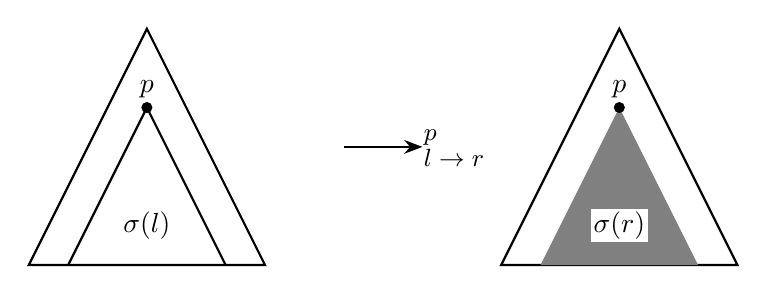
\begin{tikzpicture}[sibling distance=5em]
  \draw [thick] (0,0) -- +(3,0) -- +(1.5,3) -- cycle;
  \draw [thick] (0.5,0) -- +(1,2) -- +(2,0);

  \fill (1.5,2) circle [radius=2pt] node [above] {$p$};
  \draw (1.5,0.5) node {$\sigma(l)$};

  \draw [-{Stealth},thick] (4,1.5) -- +(1,0);
  \draw (5.1,1.4) node [above=0pt] {\small $p$};
  \draw (5.4,1.6) node [below=0pt] {\small $l\ra r$};

  \begin{scope}[xshift=60mm]
    \draw [thick] (0,0) -- +(3,0) -- +(1.5,3) -- cycle;
    \fill [gray] (0.5,0) -- +(1,2) -- +(2,0) -- cycle;

    \fill (1.5,2) circle [radius=2pt] node [above] {$p$};
    \draw (1.5,0.5) node [inner sep=1pt,fill=white] {$\sigma(r)$};
  \end{scope}  

\end{tikzpicture}
\caption{重写的树视图}
\label{f:rewriting}
\end{figure}

\begin{example}
利用例~\ref{e:add} 的重写模型$\cR$,可以得到以下重写序列,其中被重写替换的子项表达式(即重写规则左项的实例)用下划线标出:
\begin{eqnarray}
t_1 & = & \underline{\add(\s(\zero),\zero)} \lrps{}{} \s(\underline{\add(\zero,\zero)}) \lrps{}{} \s(\zero) \;\; ;\nonumber \\
t _2 & = & \underline{\add(\s^2(\zero),\s(\zero))} \lrps{}{} \s(\underline{\add(\s(\zero),\s(\zero))}) \nonumber\\ 
& & \lrps{}{} \s^2(\underline{\add(\zero,\s(\zero))}) \lrps{}{} \s^2(\s(\zero)) \;\; .\nonumber 
\end{eqnarray}
\end{example}

从上例不难看出,例~\ref{e:add} 的重写模型$\cR$定义了自然数加法的计算方式,即通过重写规则赋予了抽象函数符号$\add$自然数加法的语义。由于$\cR$不满足自然数乘法的性质,因此无法将$\add$解释为自然数乘法符号。因此,重写模型通过重写规则给函数符号赋予语义。

重写可以看作一种计算,也可以看作一种关系。

\begin{definition}[重写关系]
给定定义在词汇表$\cF$上的重写模型$\cR$,$\cR$对应的重写关系$\lrps{}{\cR}$定义为$\TFX$上的二元关系:
\begin{eqnarray}
\lrps{}{\cR} & \defeq & \{ \lb u,v\rb 
\mid \mbox{存在$p$和$(l\ra r)\in\cR$,满足$u\lrps{p}{l\ra r}v$}\}  \nonumber 
\end{eqnarray}
给定重写关系 $\lrps{}{\cR}$,它的对称闭包记作$\eqps{}{\cR}$,自反传递闭包记作 
$\lrps{*}{\cR}$,自反对称传递闭包记作$\eqps{*}{\cR}$。
\end{definition}

重写是一种\emph{非确定}的技术。重写的非确定性体现在两个方面:(1) 给定项表达式$t$,重写发生的位置$p$允许是任意的;(2) 给定项表达式$t$,重写应用的重写规则$l \ra r$允许是任意的。例如在例~\ref{e:nondet} 中,从项表达式$t$出发,产生了两条不同的重写序列。第一条序列先在位置$\rootp$(即树的根结点)进行重写,然后继续在位置$\rootp$进行重写;第二条序列则先在位置$2$(即根结点的第2个子结点)进行重写,然后继续在位置$\rootp$进行重写。

\begin{example}
\label{e:nondet}
利用例~\ref{e:add} 的重写模型$\cR$,可以得到以下重写序列:
\begin{eqnarray}
t & = & \underline{\add(\zero,\add(\zero,x))} \lrps{\rootp}{} 
\underline{\add(\zero,x)} \lrps{\rootp}{} x \nonumber \\
t & = & \add(\zero,\underline{\add(\zero,x)}) \lrps{2}{} 
\underline{\add(\zero,x)} \lrps{\rootp}{} x \nonumber 
\end{eqnarray}
\end{example}

重写过程不一定是终止的,即某项表达式$t$可以一直被重写,其过程不会停止。如例~\ref{e:nonter},利用重写模型$\cR_1$,可以得到无穷的重写序列$a\lrps{}{\cR_1}a\lrps{}{\cR_1} a \lrps{}{\cR} \ldots$;利用重写模型$\cR_2$,可以得到无穷的重写序列$f(a,b) \lrps{}{\cR_2} f(b,a) \lrps{}{\cR_2} f(a,b) \lrps{}{\cR_2} \ldots$。

\begin{example}
\label{e:nonter}
给定$\cF_1=\{a^{(0)}\}$,定义
\begin{eqnarray}
\cR_1 & = & \{a \ra a\} \; ; \nonumber
\end{eqnarray}
给定$\cF_2=\{a^{(0)},b^{(0)},f^{(2)}\}$,定义
\begin{eqnarray}
\cR_2 & = & \{f(x,y) \ra f(y,x)\} \; ; \nonumber
\end{eqnarray}
\end{example}

\begin{definition}[终止性]
\label{d:termination}
给定重写关系$\lrps{}{\cR}$,如果对任意项表达式$t$都不存在无穷的重写序列$t\lrps{}{\cR} t_1 \lrps{}{\cR} t_2 \lrps{}{\cR} \ldots$,则称重写关系$\lrps{}{\cR}$是终止的。重写模型$\cR$是终止的,当且仅当重写关系$\lrps{}{\cR}$是终止的。
\end{definition}

\begin{definition}[范式]
\label{d:normalform}
给定重写模型$\cR$,如果项表达式$s$无法应用任意重写规则$(l \ra r)\in \cR$进行重写,则称$s$是(关于$\cR$的)范式。
\end{definition}

\begin{lemma}
如果重写模型$\cR$是终止的,那么对任意项表达式$t\in\TFX$,存在范式$s\in\TFX$满足$t\lrps{*}{\cR} s$。此时称$s$是$t$(关于$\cR$)的范式,重写序列$t\lrps{*}{\cR} s$可记作$t\lrps{!}{\cR} s$。求范式的过程称作\emph{规范化}。
\end{lemma}

重写的终止性是重写领域研究的重要问题之一。给定任意一个重写模型$\cR$,判定$\cR$是否终止的问题,是一个\emph{不可判定}的问题~\cite{DBLP:conf/rta/Dauchet89,tech1978}。重写模型的终止性问题不是本文讨论的内容,在此不详述,更多探讨可参考~\inlinecite{terese,DBLP:conf/rta/1995,DBLP:journals/iandc/GeserHWZ07,DBLP:journals/tcs/Payet08,DBLP:journals/tcs/Lescanne94,DBLP:conf/tlca/JouannaudL15}。

由于重写的非确定性,即使重写模型是终止的,任意项表达式的范式也不一定是唯一的。如例~\ref{e:diffnorm},根据$\cR$,有$a\lrps{!}{\cR} b$以及$a \lrps{!}{\cR}c$,即$b$和$c$都是关于$\cR$的$a$的范式,可见$a$的范式并不唯一。

\begin{example}
\label{e:diffnorm}
给定$\cF=\{a^{(0)},b^{(0)},c^{(0)}\}$,定义
\begin{eqnarray}
\cR & = & \{a \ra b\; , a\ra c\} \; \mbox{。} \nonumber
\end{eqnarray}
\end{example}

\begin{definition}[合流性]
\label{d:confluence}
给定重写关系$\lrps{}{\cR}$,如果对任意满足$u\rlps{*}{\cR} s \lrps{*}{\cR} v$的项表达式$s,u,v$,都存在$t$使$u\lrps{*}{\cR} t \rlps{*}{\cR} v$,则称$\lrps{}{\cR}$是合流的。重写模型$\cR$是合流的,当且仅当重写关系$\lrps{}{\cR}$是合流的。
\end{definition}

重写的合流性也是重写领域研究的重要问题之一。给定任意一个重写模型$\cR$,判定$\cR$是否合流的问题,也是一个不可判定的问题~\cite{DBLP:journals/ipl/Jacquemard03}。与终止性类似,重写模型的合流性问题不是本文讨论的内容,在此不详述,更多探讨可参考~\inlinecite{terese,newman42,hindley1964church,DBLP:journals/jacm/Rosen73,knuth70,DBLP:conf/rta/Oostrom08,DBLP:journals/jar/ZanklFM15,DBLP:conf/csl/LiuJO15,DBLP:conf/rta/LiuDJ14}。

把重写看作计算的过程,终止性保证计算结果存在,而合流性保证计算结果唯一,即计算过程的非确定性不影响计算结果的确定性。

\begin{lemma}
如果重写模型$\cR$是终止的且合流的,那么任意项表达式$t$关于$\cR$的范式存在且唯一,记作$\nf{t}{\cR}$。在$\cR$已知的情况下,简记作$\nf{t}{}$。
\end{lemma}



\subsection{等式规则与等价关系}

重写规则是有方向性的,因此重写是不可逆的过程。给定$s\lrps{}{\cR}t$,$s$和$t$处于不等价的关系。然而在某些情况下,我们需要描述两个项表达式之间等价的关系。例如针对例~\ref{e:add} 的重写模型,项表达式$\add(x,\zero)$已经是自身的范式,$\add(x,\zero) = \nf{\add(x,\zero)}{}$。但正如之前的描述,我们想赋予$\add$自然数加法的语义。我们知道交换律是自然数加法具有的性质,在此意义上,我们认为项表达式$\add(x,\zero)$应该可以进一步化简为$x$。因此交换律的语义应该以形如$\add(x,y)\ra\add(y,x)$的重写规则被加入到该重写模型中。然而,从例~\ref{e:nonter} 的$\cR_2$可以看出,这种形式的重写规则会破坏重写模型的终止性。

为此,需要引入等式规则与等价关系的概念。

\begin{definition}[等式规则]
\label{d:eq}
给定词汇表$\cF$,一条等式规则是由项表达式$l,r\in\TFX$组成的无序对(无序二元组),记作$l\sim r$。
\end{definition}

\begin{definition}[等价模型]
\label{d:eq-sys}
给定词汇表$\cF$,等价模型是一个由若干等式规则组成的集合$\cE = \{l_i \sim r_i\}_i$。
\end{definition}

由于等式规则是无序对,因此$l\sim r$等同于$r\sim l$。$(l\sim r)\in\cE$当且仅当$(r\sim l)\in\cE$。

\begin{example}
\label{e:add-ac}
假定$\cF = \{\add^{(2)}\}$。可定义以下等价模型:
\begin{eqnarray}
\cE = \{ &  & \add(x, y) \sim \add(y,x) \; , \nonumber \\
         &  & \add(\add(x,y), z) \sim \add(x,\add(y,z)) \;\;\; \}\mbox{。} \nonumber
\end{eqnarray}
\end{example}

例~\ref{e:add-ac} 的规则分别定义了函数符号$\add$的交换律和结合律。

应用等式规则的方式与应用重写规则的方式类似:

\begin{definition}[等价]
\label{d:equality}
给定等价模型$\cE$,项表达式$u,v\in\TFX$,位置$p\in\Pos{u}$,等式规则$(l \sim r) \in \cE$。如果存在代换$\sigma$满足$u|_p = \sigma(l)$以及$v=u[\sigma(r)]_p$,则称$u$和$v$在位置$p$关于等式规则$l\sim r$等价,记作$u\eqps{p}{l\sim r} v$。记号中的$p$和$l\sim r$可忽略不写。
\end{definition}

记号$\eqps{}{}$表明了应用等式规则的过程是个对称、可逆的过程。

\begin{example}
利用例~\ref{e:add-ac} 的等价模型,可得到以下等价序列:
\begin{eqnarray}
& & \add(\add(x,y),z) \eqps{1}{} \add(\add(y,x),z) \eqps{\rootp}{} \add(y,\add(x,z)) \eqps{\rootp}{} \add(\add(x,z),y) \mbox{。}\nonumber 
\end{eqnarray}
\end{example}

\begin{definition}[等价关系]
\label{d:equiv}
给定定义在词汇表$\cF$上的等价模型$\cE$,$\cE$对应的等价关系$\eqps{}{\cE}$定义为$\TFX$上的二元关系:
\begin{eqnarray}
\eqps{}{\cE} & \defeq & \{ \lb u,v\rb 
\mid \mbox{存在$p$和$(l\sim r)\in\cE$,满足$u\eqps{p}{l\sim r}v$}\}  \nonumber 
\end{eqnarray}
给定等价关系 $\eqps{}{\cE}$,它的对称闭包是它自身,自反传递闭包记作 
$\eqps{*}{\cE}$。
\end{definition}

由于等价关系是对称的,任意等价关系$u\eqps{}{\cE}v$都可以扩展成一个无穷等价序列$u\eqps{*}{\cE}v$。因此区分等价关系$\eqps{}{\cE}$及其自反传递闭包$\eqps{*}{\cE}$并无意义。我们将$u\eqps{*}{\cE}v$记作$u=_{\cE}v$。

\section{重写模型的扩展}

\subsection{模重写}

等价关系为抽象的函数符号赋予了“等价”的语义。等价关系的引入,是为了增强重写的能力。\emph{模重写}技术的目的就是定义一种二者融合的方式。

\begin{definition}[模重写模型]
\label{d:rewsys-modulo}
给定词汇表$\cF$,模重写模型是一个由重写模型$\cR$和等价模型$\cE$组成的有序对(二元组),记作$\cR_{\cE} \defeq \lb \cR, \cE \rb$。
\end{definition}

\begin{definition}[模重写]
\label{d:rewriting-modulo}
给定模重写模型$\RE$,项表达式$u,v\in\TFX$,位置$p\in\Pos{u}$,重写规则$(l \ra r) \in \cR$。如果存在代换$\sigma$满足$u|_p =_{\cE} \sigma(l)$以及$v=u[\sigma(r)]_p$,则称$u$在位置$p$应用重写规则$l\ra r$模重写为$v$,记作$u\lrps{p}{(l\ra r)_{\cE}} v$。记号中的$p$和$(l\ra r)_{\cE}$可忽略不写。
\end{definition}

重写技术替换的是项表达式$u$中存在的规则左项的实例$\sigma(l)$,而模重写技术替换的则是$u$中与规则左项实例$\sigma(l)$关于$\cE$等价的子项表达式。这使得重写过程得以“利用”各函数符号的等价语义。

\begin{example}
\label{e:add-ac-mod}
假定$\cF = \{\zero^{(0)}, \s^{(1)}, \add^{(2)}\}$。可定义模重写模型$\RE$,其中:
\begin{eqnarray}
\cR = \{ &  & \add(\zero, y) \ra y \; , \nonumber \\
         &  & \add(\s(x), y) \ra \s(\add(x,y)) \;\;\; \}\;\; ; \nonumber \\
\cE = \{ &  & \add(x, y) \sim \add(y,x) \; , \nonumber \\
         &  & \add(\add(x,y), z) \sim \add(x,\add(y,z)) \;\;\; \}\mbox{。} \nonumber         
\end{eqnarray}
可得到以下模重写序列:
\begin{eqnarray}
t_1 & = & \underline{\add(x,\s(\zero))} \lrps{}{} \s(\underline{\add(\zero,x)}) \lrps{}{} \s(x) \;\; ;\nonumber \\
t _2 & = & \underline{\add(\add(x,\s(\zero)),y)} \lrps{}{} \s(\underline{\add(\zero,\add(x,y))}) 
\lrps{}{} \s(\add(x,y)) \;\; \mbox{。}\nonumber 
\end{eqnarray}
\end{example}

类似于重写,我们可以定义模重写对应的模重写关系、终止性、范式和合流性。

\begin{definition}[模重写关系]
给定定义在词汇表$\cF$上的模重写模型$\RE$,$\RE$对应的模重写关系$\lrps{}{\RE}$定义为$\TFX$上的二元关系:
\begin{eqnarray}
\lrps{}{\RE} & \defeq & \{ \lb u,v\rb 
\mid \mbox{存在$p$和$(l\ra r)\in\cR$,满足$u\lrps{p}{(l\ra r)_{\cE}}v$}\}  \nonumber 
\end{eqnarray}
给定模重写关系 $\lrps{}{\RE}$,它的对称闭包记作$\eqps{}{\RE}$,自反传递闭包记作 
$\lrps{*}{\RE}$,自反对称传递闭包记作$\eqps{*}{\RE}$。
\end{definition}

\begin{definition}
给定模重写关系$\lrps{}{\RE}$,如果对任意项表达式$t$都不存在无穷的模重写序列$t\lrps{}{\RE} t_1 \lrps{}{\RE} t_2 \lrps{}{\RE} \ldots$,则称模重写关系$\lrps{}{\RE}$是终止的。模重写模型$\RE$是终止的,当且仅当模重写关系$\lrps{}{\RE}$是终止的。
\end{definition}

\begin{definition}
给定模重写模型$\RE$,如果项表达式$s$无法应用任意重写规则$(l \ra r)\in \cR$进行模重写,则称$s$是(关于$\RE$的)范式。
\end{definition}

\begin{lemma}
如果模重写模型$\RE$是终止的,那么对任意项表达式$t\in\TFX$,存在范式$s\in\TFX$满足$t\lrps{*}{\RE} s$。此时称$s$是$t$(关于$\RE$)的范式,模重写序列$t\lrps{*}{\RE} s$可记作$t\lrps{!}{\RE} s$。
\end{lemma}

\begin{definition}
给定模重写关系$\lrps{}{\RE}$,如果对任意满足$u\rlps{*}{\RE} s \lrps{*}{\RE} v$的项表达式$s,u,v$,都存在$t$和$t'$使$u\lrps{*}{\RE} t =_{\cE} t' \rlps{*}{\RE} v$,则称$\lrps{}{\RE}$是合流的。模重写模型$\RE$是合流的,当且仅当模重写关系$\lrps{}{\RE}$是合流的。
\end{definition}

\begin{lemma}
如果模重写模型$\RE$是终止的且合流的,那么任意项表达式$t$关于$\RE$的范式存在且关于$\cE$等价。也就是说,如果$t\lrps{!}{\RE} s_1$,$t\lrps{!}{\RE} s_2$,那么$s_1 =_{\cE} s_2$。 此时也可称$t$关于$\RE$的范式关于$=_{\cE}$唯一,将任一范式记作$\nf{t}{\RE}$。在$\RE$已知的情况下,简记作$\nf{t}{}$。
\end{lemma}

模重写技术可以看作是将重写技术中的语法等价(相等关系$=$)扩展为语义等价(等价关系$=_{\cE}$)。重写模型是模重写模型的等价关系$=_{\cE}$为空时的特殊情况,即$\cR = \cR_{\emptyset}$。关于模重写的终止性和合流性的研究,可参考\inlinecite{terese,DBLP:conf/cade/JouannaudM84,DBLP:journals/tcs/JouannaudM92,DBLP:journals/ijsi/JouannaudT08,DBLP:conf/rta/Jouannaud06,DBLP:journals/tcs/JouannaudL12,DBLP:journals/siamcomp/JouannaudK86}。


\subsection{条件重写}

对于标准的重写技术,触发重写的条件是通过模式匹配体现的。假如给定形如$f(x)$的项表达式,我们希望当$x\ge 2$时,$f(x)$可以重写为$a$;当$x<2$时,$f(x)$可以重写为$b$。那么根据例~\ref{e:add},我们需要增加如下规则:
\begin{eqnarray}
f(\s^2(x)) & \ra & a \nonumber \\
f(\zero)  & \ra & b \nonumber \\
f(\s(\zero)) & \ra & b \nonumber
\end{eqnarray}
如果判断是否满足$x\ge 3$,则右项为$b$的规则需要增加至3条;以此类推,如果判断是否满足$x\ge n$,右项为$b$的规则需要增加至n条。这就给设计规则的过程带来极大不便。

给重写规则增加条件约束,则可以大大地增加重写规则的表达能力。例如我们希望可以通过以下形式的规则来表示上述的情况:
\begin{eqnarray}
f(x) & \ra & a ~~\mbox{ if }~~ x\ge \s^2(\zero) \nonumber \\
f(x)  & \ra & b ~~\mbox{ if }~~ x < \s^2(\zero) \nonumber 
\end{eqnarray}

\begin{definition}[条件重写规则]
\label{d:crule}
给定词汇表$\cF$,条件重写规则由重写规则和若干等式构成,形如
\begin{eqnarray}
l \ra r & \Dla & u_1 = v_1 \land \ldots \land u_n = v_n \;\; ,\nonumber
\end{eqnarray}
其中$l,r\in\TFX$,对$1\le i\le n$有$u_i,v_i\in\TFX$。其中$l$称作该条件重写规则的左项,$r$称作该条件重写规则的右项,$u_i = v_i$称作该条件重写规则的条件约束。
\end{definition}

\begin{definition}[条件重写模型]
\label{d:crewrite-sys}
给定词汇表$\cF$,条件重写模型是一个由若干条件重写规则组成的集合$\cR = \{l_i \ra r_i \Dla C_i \}_i$。
\end{definition}

\begin{example}
\label{e:cond}
假定$\cF = \{\zero^{(0)}, \s^{(1)}, \add^{(2)}, f^{(2)}, a^{(0)}, b^{(0)}, \true^{(0)}, \false^{(0)}, \mynot^{(1)}, \lessthan^{(2)} \}$。可定义以下条件重写模型:
\begin{eqnarray}
\cR = \{ &  & f(x) \ra a \;\Dla\; \mynot(\lessthan(x,\s^2(\zero))) = true \; , \nonumber \\
         &  & f(x) \ra b \;\Dla\; \lessthan(x,\s^2(\zero)) = ture \;\;\;\;\; \}\mbox{。} \nonumber
\end{eqnarray}
\end{example}

例~\ref{e:cond} 中的两条规则对应了本小节开头提出的重写需求。

虽然我们给出了条件重写规则的形式,但是其语义并不清晰。条件重写规则里的条件约束$u_i=v_i$,是代表$u_i$和$v_i$语法上的相等呢?是代表$u_i\eqps{*}{}v_i$呢?是代表存在$t$使$u_i\lrps{*}{}t\rlps{*}{}v_i$呢?还是$u_i\lrps{*}{}v_i$呢?关于条件约束的不同语义解释有多种讨论~\cite{brand1978completeness,DBLP:journals/jcss/BergstraK86,DBLP:conf/cade/DershowitzOS88},这里我们采用最常用的实现方法:
存在$t$使$u_i\lrps{*}{}t\rlps{*}{}v_i$。

\begin{definition}[条件重写]
\label{d:crewriting}
给定条件重写模型$\cR$,项表达式$u,v\in\TFX$,位置$p\in\Pos{u}$,条件重写规则$(l \ra r \Dla C_i) \in \cR$。如果存在代换$\sigma$满足$u|_p = \sigma(l)$,$v=u[\sigma(r)]_p$,以及对任意$(u_j = v_j)\in C_i$存在$t_j$使$u_j\lrps{*}{} t_j \rlps{*}{} v_j$, 则称$u$在位置$p$应用条件重写规则$l\ra r \Dla C_i$重写为$v$,记作$u\lrps{p}{l\ra r} v$。记号中的$p$和$l\ra r$可忽略不写。
\end{definition}

条件重写的意思是,被重写的子项表达式不仅需要是重写规则左项$l$的实例,且其对应的代换$\sigma$需要满足该规则的所有条件约束。

针对例~\ref{e:cond},为了实现条件约束的求解,还需要加入以下规则:
\begin{eqnarray}
\lessthan(x,\zero) & \ra & \false \nonumber \\
\lessthan(\zero,\s(y)) & \ra & \true \nonumber \\
\lessthan(\s(x),\s(y)) & \ra & \lessthan(x,y) \nonumber \\
\mynot(\false) & \ra & \true \nonumber \\
\mynot(\true) & \ra & \false \;\;\mbox{。} \nonumber 
\end{eqnarray}

重写模型对应于条件重写模型中所有条件约束均为空的特殊情况。重写模型的相关概念,包括重写关系、终止性、范式及合流性,均可自然地扩展成条件重写模型的对应概念,在此不再赘述。给定任意模重写模型$\RE$,将其中的重写模型$\cR$替换成条件重写模型,则得到\emph{条件模重写}模型及其相关概念。


\section{规范化条件重写模型}

在模重写和条件重写的基础上,本文提出一种新的重写模型扩展,叫\emph{规范化条件重写模型}。

条件重写模型在应用某条重写规则时,需要判断其条件约束是否成立,即是否存在$t$使$u_i\lrps{*}{}t\rlps{*}{}v_i$,这个过程是不可判定的~\cite{DBLP:journals/ipl/Jacquemard03}。理想的做法是通过$u_i$和$v_i$的范式来确定条件是否成立,即判断是否有${\nf{u_i}{}} = {\nf{v_i}{}}$。此时,只需要在语法上判断是否相等即可。这就要求该条件重写模型是终止的,或者至少要求用于求范式的重写规则是终止的~\cite{DBLP:conf/cade/DershowitzOS88,DBLP:journals/tcs/DershowitzO90,DBLP:conf/rta/BertlingG89}。另一方面,在例~\ref{e:cond} 中,注意到用于求解条件约束的规则与描述需求的规则(即$f(x)\ra a$与$f(x)\ra b$)相对独立。规则$f(x)\ra a$和$f(x)\ra b$用于赋予模型语义,而其它规则则用于辅助定义$f(x)\ra a$和$f(x)\ra b$。这当中存在层次关系,而属于同一个重写规则集使得该有的区别模糊不清,这从概念上和技术上都是欠妥的。

本文提出的规范化(条件)重写模型,则是基于上述考虑,将(条件)模重写模型进一步划分层次。


\begin{definition}[规范化重写模型]
\label{d:normalrew-sys}
给定词汇表$\cF$,规范化重写模型是一个由重写模型$\cR,\cS$和等价模型$\cE$组成的三元组,记作$\RSE \defeq \lb \cR, \cS, \cE \rb$。其中由$\cS$和$\cE$组成的模重写模型$\SE$必须满足终止性和合流性。
\end{definition}

重写不一定是终止的,因此不能将任意重写模型的重写过程看作是化简的过程。例如规则$a\ra f(a)$会将项表达式$a$重写为更加复杂的表达式。但是当重写模型具有终止性时,重写过程就可以看作是一个化简的过程。规范化重写模型$\RSE$要求$\SE$是终止且合流的,使得$\SE$可看作一个良定义的化简函数:计算结果(范式)存在且唯一。因此,重写模型$\cS$可称作\emph{化简模型},其对应的重写规则可称作\emph{化简规则}。

\begin{definition}[规范化重写]
\label{d:normalrewriting}
给定规范化重写模型$\RSE$,项表达式$u,v\in\TFX$,重写规则$(l \ra r) \in \cR$。如果存在位置$p$和项表达式$s,t$满足
${\nf{u}{\SE}} =_{\cE} s \lrps{p}{l\ra r} t$且$v = {\nf{t}{\SE}}$,则称$u$应用重写规则$l\ra r$规范化重写为$v$,记作$u\lrps{}{(l\ra r)_{\cS\cE}} v$。记号中的$(l\ra r)_{\cS\cE}$在不存在二义性时可忽略不写。
\end{definition}

简单地说,如果$u\lrps{}{(l\ra r)_{\cS\cE}}v$,则$u$和$v$之间存在关系
$u \lrps{!}{\SE} {\nf{u}{\SE}} =_{\cE} s \lrps{p}{l\ra r} t \lrps{!}{\SE} {\nf{t}{\SE}} = v$。从技术上看,给定项表达式$u$,要想对$u$进行规范化重写,需要先对$u$进行规范化,得到$u$关于$\SE$的范式$\nf{u}{\SE}$。然后在$\nf{u}{\SE}$关于$=_{\cE}$的等价类中选定项表达式$s$,对其进行重写得到项表达式$t$。最后对$t$进行规范化得到其关于$\SE$的范式$\nf{t}{\SE}$。

规范化重写技术在应用重写规则前,要求项表达式必须是范式。在应用重写规则后,又显式地进行规范化,使最终得到的项表达式成为范式。这就保证对于任意规范化重写序列$u_0 \lrps{}{} u_1 \lrps{}{} \ldots \lrps{}{} u_n$,对任意$i\in [1,n]$满足$u_i$是关于$\SE$的范式,即重写序列中的项表达式始终处于“最简”形式。

规范化重写模型通过对规则分类,使模型的语义更加清晰:$\cE$描述与等价相关的语义,$\cS$描述与函数计算、形式简化相关的语义,$\cR$描述最核心的、用户关心的语义。

\begin{example}
\label{e:river}
假定$\cF = \{\comp^{(2)}, \farmer^{(1)}, \wolf^{(1)}, \lamb^{(1)}, \grass^{(1)}, \lhs^{(0)}, \rhs^{(0)}, \change^{(1)} \}$,其中函数符号$\comp$采用中缀记法,即$x\comp y$表示$\comp(x,y)$。可定义规范化重写模型$\RSE$,其中:
\begin{eqnarray}
\cE = \{ &  & x\comp y \sim y\comp x \; , \nonumber \\
         &  & (x\comp y) \comp z \sim x \comp (y\comp z)  \;\;\;\;\; \} \; ; \nonumber \\
\cS = \{ &  & \change(\lhs) \ra \rhs \; , \nonumber \\
         &  & \change(\rhs) \ra \lhs \;\;\;\;\; \} \; ; \nonumber \\
\cR = \{ &  & \farmer(x) \ra_1 \farmer(\change(x)) \; , \nonumber \\
         &  & \farmer(x)\comp \wolf(x) 
         \ra_2 \farmer(\change(x))\comp\wolf(\change(x)) \; , \nonumber \\
         &  & \farmer(x)\comp \lamb(x) 
         \ra_3 \farmer(\change(x))\comp\lamb(\change(x)) \; , \nonumber \\ 
         &  & \farmer(x)\comp \grass(x) 
         \ra_4 \farmer(\change(x))\comp\grass(\change(x)) \; \} \mbox{。}\nonumber
\end{eqnarray}
可得到以下规范化重写序列:
\begin{eqnarray}
t & = & \farmer(\lhs) \comp \wolf(\lhs) \comp 
        \lamb(\lhs) \comp \grass(\lhs) \nonumber \\
  & \lrps{}{3} & \farmer(\rhs) \comp \lamb(\rhs) \comp 
        \wolf(\lhs) \comp \grass(\lhs) \nonumber \\
  & \lrps{}{1} & \farmer(\lhs) \comp \lamb(\rhs) \comp 
        \wolf(\lhs) \comp \grass(\lhs) \nonumber \\
  & \lrps{}{2} & \farmer(\rhs) \comp \wolf(\rhs) \comp 
        \lamb(\rhs) \comp \grass(\lhs) \nonumber \\    
  & \lrps{}{3} & \farmer(\lhs) \comp \lamb(\lhs) \comp 
        \wolf(\rhs) \comp \grass(\lhs) \nonumber \\    
  & \lrps{}{4} & \farmer(\rhs) \comp \grass(\rhs) \comp 
        \wolf(\rhs) \comp \lamb(\lhs) \nonumber \\     
  & \lrps{}{1} & \farmer(\lhs) \comp \grass(\rhs) \comp 
        \wolf(\rhs) \comp \lamb(\lhs) \nonumber \\                  
  & \lrps{}{3} & \farmer(\rhs) \comp \lamb(\rhs) \comp 
        \wolf(\rhs) \comp \grass(\rhs) \; \mbox{。} \nonumber
\end{eqnarray}
\end{example}

例~\ref{e:river} 描述的是农夫过河的问题。$\lhs$和$\rhs$分别表示河的左岸和右岸;$\farmer(x)$、$\wolf(x)$、$\lamb(x)$和$\grass(x)$分别表示农夫、狼、羊和草当前所处位置为河的$x$岸;$\change(x)$表示$x$岸的对岸;$\comp$作为连接符构成农夫、狼、羊和草在任一时刻的状态,如$\farmer(\lhs) \comp \lamb(\lhs) \comp \wolf(\rhs) \comp \grass(\lhs)$
表示当前状态为农夫在左岸、羊在左岸、狼在右岸、草在左岸。$\cE$的等价规则分别表示函数符号$\comp$具有交换律和结合律,因此$\comp$连接的多个项表达式构成了一个多重集合,其中的括号可以省略。$\cS$的重写规则定义了化简$\change$的方式。$\cR$的四条规则定义了系统状态发生改变的四种方式:(1) 农夫独自一人过河;(2) 农夫带着狼过河;(3) 农夫带羊过河;(4) 农夫带草过河。$\cR$的规则用数字进行了编号。例~\ref{e:river} 的重写序列描述了一种可能的方案,从农夫、狼、羊和草都处于左岸的初始状态,变成四者都处于右岸的状态。序列中用右箭头的数字下标表示规范化重写应用的规则编号。

\begin{definition}[规范化重写关系]
给定定义在词汇表$\cF$上的规范化重写模型$\RSE$,$\RSE$对应的规范化重写关系$\lrps{}{\RSE}$定义为$\TFX$上的二元关系:
\begin{eqnarray}
\lrps{}{\RSE} & \defeq & \{ \lb u,v\rb 
\mid \mbox{存在$(l\ra r)\in\cR$,满足$u\lrps{}{(l\ra r)_{\cS\cE}}v$}\}  \nonumber 
\end{eqnarray}
给定规范化重写关系 $\lrps{}{\RSE}$,它的对称闭包记作$\eqps{}{\RSE}$,自反传递闭包记作 
$\lrps{*}{\RSE}$,自反对称传递闭包记作$\eqps{*}{\RSE}$。
\end{definition}

类似地,条件约束可以增加规范化重写模型的表达能力,扩展得到\emph{规范化条件重写模型}。


\begin{definition}[规范化条件重写模型]
\label{d:cnormalrew-sys}
给定词汇表$\cF$,规范化条件重写模型是一个由条件重写模型$\cR,\cS$和等价模型$\cE$组成的三元组,记作$\RSE \defeq \lb \cR, \cS, \cE \rb$。其中由$\cS$和$\cE$组成的条件模重写模型$\SE$必须满足终止性和合流性。
\end{definition}

上文已经提到,条件重写模型是重写模型的一种自然扩展。规范化条件重写模型仅仅是将规范化重写模型$\lb \cR, \cS, \cE\rb$中的标准重写模型$\cR$和$\cS$扩展为条件重写模型,且同样对$\SE$的终止性和合流性有要求。

虽然在形式上看,规范化条件重写模型只是简单地将重写规则替换为条件重写规则。但从语义解释上,却与简单的替换有所不同。

\begin{definition}[规范化条件重写]
\label{d:cnormalrewriting}
给定规范化条件重写模型$\RSE$,项表达式$u,v\in\TFX$,条件重写规则$(l \ra r \Dla C_i) \in \cR$。如果存在位置$p$、代换$\sigma$和项表达式$s,t$满足:
\begin{enumerate}[(i)]
\item ${\nf{u}{\SE}} =_{\cE} s$;    
\item $s|_p = \sigma(l)$,$t = s[\sigma(r)]_p$;
\item 对任意$(u_j = v_j)\in C_i$,存在$w_j$使$u_j\lrps{*}{\SE} w_j \rlps{*}{\SE} v_j$;
\item $v = {\nf{t}{\SE}}$;
\end{enumerate}
则称$u$应用条件重写规则$l\ra r \Dla C_i$规范化条件重写为$v$,记作$u\lrps{}{(l\ra r)_{\cS\cE}} v$。记号中的$(l\ra r)_{\cS\cE}$在不存在二义性时可忽略不写。
\end{definition}
 

与规范化重写类似,如果$u\lrps{}{(l\ra r)_{\cS\cE}}v$,则$u$和$v$之间存在关系
$u \lrps{!}{\SE} {\nf{u}{\SE}} =_{\cE} s \lrps{p}{l\ra r} t \lrps{!}{\SE} {\nf{t}{\SE}} = v$。
但需要注意其中的条件重写步骤$s\lrps{p}{l\ra r}t$,它判断条件约束$u_j=v_j$是否成立时,不是递归地使用模型$\RSE$,而是直接使用$\SE$。也就是说,$u_j$和$v_j$需要满足
$u_j\lrps{*}{\SE} w_j \rlps{*}{\SE} v_j$而不是$u_j\lrps{*}{\RSE} w_j \rlps{*}{\RSE} v_j$。由于条件模重写模型$\SE$是终止且合流的,$u_j\lrps{*}{\SE} w_j \rlps{*}{\SE} v_j$可以进一步简化为${\nf{u_j}{\SE}} =_{\cE} {\nf{v_j}{\SE}}$,这就在一定程度上解决了本小节开头提出的不可判定性问题,使规范化条件重写从技术上可以被实现。

与规范化重写类似,从技术上看,规范化条件重写也必须经过规范化、条件重写、规范化三个过程。这保证了规范化条件重写序列中的任意项表达式都始终处于“最简”形式。

\begin{definition}[规范化条件重写关系]
给定定义在词汇表$\cF$上的规范化条件重写模型$\RSE$,$\RSE$对应的规范化条件重写关系$\lrps{}{\RSE}$定义为$\TFX$上的二元关系:
\begin{eqnarray}
\lrps{}{\RSE} & \defeq & \{ \lb u,v\rb 
\mid \mbox{存在$(l\ra r)\in\cR$,满足$u\lrps{}{(l\ra r)_{\cS\cE}}v$}\}  \nonumber 
\end{eqnarray}
给定规范化条件重写关系 $\lrps{}{\RSE}$,它的对称闭包记作$\eqps{}{\RSE}$,自反传递闭包记作 
$\lrps{*}{\RSE}$,自反对称传递闭包记作$\eqps{*}{\RSE}$。
\end{definition}

\begin{example}
\label{e:cnormalrew}
假定$\cF = \{\zero^{(0)}, \s^{(1)}, f^{(2)}, a^{(0)}, b^{(0)}, \true^{(0)}, \false^{(0)}, \mynot^{(1)}, \lessthan^{(2)} \}$。可定义规范化条件重写模型$\RSE$,其中:
\begin{eqnarray}
\cE = \phantom{\{} & & \emptyset \; ; \nonumber \\
\cS = \{ & & \lessthan(x,\zero)  \ra  \false \; , \nonumber \\
         & & \lessthan(\zero,\s(y))  \ra  \true \; , \nonumber \\
         & & \lessthan(\s(x),\s(y))  \ra  \lessthan(x,y) \; , \nonumber \\
         & & \mynot(\false) \ra \true \; , \nonumber \\
         & & \mynot(\true) \ra  \false \;\;\;\;\;\;\;\qquad\quad\quad\qquad\quad \} \; ; \nonumber \\
\cR = \{ &  & f(x) \ra a \;\Dla\; \mynot(\lessthan(x,\s^2(\zero))) = true \; , \nonumber \\
         &  & f(x) \ra b \;\Dla\; \lessthan(x,\s^2(\zero)) = ture \;\;\;\;\;\qquad \}\mbox{。} \nonumber
\end{eqnarray}
\end{example}

例~\ref{e:cnormalrew} 的规范化条件重写模型对应例~\ref{e:cond}(及其新增规则)的条件重写模型。


\begin{example}
\label{e:clock}
假定$\cF = \{\zero^{(0)}, \s^{(1)}, \add^{(2)}, \clock^{(1)}, \broken^{(0)}, \true^{(0)}, \false^{(0)}, \mynot^{(1)}, \lessthan^{(2)} \}$。可定义规范化条件重写模型$\RSE$,其中:
\begin{eqnarray}
\cE = \{ &  & \add(x, y) \sim \add(y,x) \; , \nonumber \\
         &  & \add(\add(x,y), z) \sim \add(x,\add(y,z)) \;\;\; \}\; ;
         \nonumber \\
\cS = \{ &  & \add(\zero, y) \ra y \; , \nonumber \\
         &  & \add(\s(x), y) \ra \s(\add(x,y)) \; , \nonumber \\
         & & \lessthan(x,\zero)  \ra  \false \; , \nonumber \\
         & & \lessthan(\zero,\s(y))  \ra  \true \; , \nonumber \\
         & & \lessthan(\s(x),\s(y))  \ra  \lessthan(x,y) \;\;\; \} \; ;\nonumber \\
\cR = \{ &  & \clock(x) \ra_1 \clock(\add(x,\s(\zero))) 
              \;\Dla\; \lessthan(x,\s^{11}(\zero)) = \true \; , \nonumber \\
         &  & \clock(x) \ra_2 \clock(\zero) 
              \;\Dla\; \lessthan(x,\s^{11}(\zero)) = \false \; , \nonumber \\  
         &  & \clock(x) \ra_3 \broken  
              \;\;\;\qquad\qquad\qquad\qquad\qquad\qquad\qquad\qquad\qquad \}\mbox{。} \nonumber          
\end{eqnarray}
可得到以下规范化条件重写序列:
\begin{eqnarray}
t & = & \clock(\s^0(\zero)) \lrps{}{1} \clock(\s^1(\zero))
        \lrps{}{1} \clock(\s^2(\zero))
        \lrps{}{1} \clock(\s^3(\zero)) \nonumber \\
  &   & \lrps{}{1} \ldots
        \lrps{}{1} \clock(\s^{11}(\zero))
        \lrps{}{2} \clock(\s^0(\zero))
        \lrps{}{1} \clock(\s^1(\zero))       
        \lrps{}{1} \ldots \; ;
        \nonumber \\
t & = & \clock(\s^0(\zero)) \lrps{}{1} \clock(\s^1(\zero))
        \lrps{}{1} \clock(\s^2(\zero))
        \lrps{}{3} \broken \; ; \nonumber \\
t & = & \clock(\s^0(\zero)) \lrps{}{1} \clock(\s^1(\zero))
        \lrps{}{1} \clock(\s^2(\zero))
        \lrps{}{1} \clock(\s^3(\zero)) \nonumber \\
  &   & \lrps{}{1} \ldots
        \lrps{}{1} \clock(\s^{11}(\zero))
        \lrps{}{3} \broken \; \mbox{。}
        \nonumber
\end{eqnarray}
\end{example}

例~\ref{e:clock} 描述的是一个只显示时针读数(0--11)的时钟,且这个时钟随时可能损坏。函数符号$\zero$、$\s$和$\add$用于表示自然数及自然数加法,之前已详细介绍,在此不再赘述;函数符号$\true$、$\false$分别表示命题为真和命题为假,$\mynot$表示逻辑“非”运算,$\lessthan(x,y)$表示命题“x小于y”,这四个函数符号用于定义重写规则的条件约束;$\clock(x)$表示时钟当前读数为$x$;$\broken$表示时钟当前已损坏。$\cE$的等价规则分别表示自然数加法$\add$的交换律和结合律。化简模型$\cS$包含两部分,前两条规则定义了$\add$的语义,即其计算方式;后三条规则定义了$\lessthan$的语义,即如何计算命题“x小于y”的真值。$\cR$的重写规则定义了系统状态发生改变的三种方式:规则1表示,如果时钟当前读数$x$小于11,则下一个状态的读数为$x+1$;规则2表示,如果时钟当前读数$x$不小于11,则下一个状态的读数为0(归零);规则3表示,无论时钟当前读数是多少,下一个状态时钟可能损坏。例~\ref{e:clock} 的重写序列描述了从初始状态(时钟读数为0)开始,该时钟可能发生的(其中)三种事件序列,其中箭头下标的数字表示该规范化条件重写应用的规则编号。序列1表示时钟读数从0递增至11,然后归零,周而复始,该时钟始终保持正常运作。序列2表示时钟读数从0递增至2,然后发生损坏。序列3表示时钟读数从0递增至11,然后发生损坏。

从例~\ref{e:clock} 可以看出,时钟状态是观察者关心的行为,而自然数加法、命题真值的计算只是为描述时钟状态服务,观察者并不关心。从建模的角度来看,将所有规则平等看待,非常不利于建模人员或其它模型使用者理解模型的语义。规范化条件重写模型以一种划分的方式,将模型的主要语义和辅助语义予以区分。

\section{相关工作}
\todo{进行与normalized rewriting, normal rewriting及rewriting logic的对比。}


\chapter{嵌入式系统的建模与验证}
\chapter{C 语言程序终止性的自动验证}
\chapter{结束语}
\label{cha:conclusion}

\section{工作总结}

针对现代嵌入式系统结构复杂、行为复杂所引发的形式化建模与验证问题,本文基于重写理论,完成了以下工作:

\begin{enumerate}
\item 
针对嵌入式系统中硬件的并发行为与软件的顺序行为并存的异构性特征进行研究,提出了规范化条件重写模型。将硬件的并发行为抽象成不确定性行为,将软件的顺序行为抽象成确定性行为,基于模重写模型、条件重写模型以及 Nipkow 在高阶重写中使用的 $\beta\eta$ 规范化过程,本文提出的规范化条件重写模型,利用等式规则描述系统的结构特征及状态等价关系,利用条件约束描述系统的控制流特征,利用化简规则描述系统的确定性行为,利用重写规则描述系统的不确定性行为。本文对重写模型的规则应用策略进行扩展,定义了在多种规则共存的情况下,确定性行为与不确定性行为的协作方式,且保证了重写规则触发时条件约束的可判定性。规范化条件重写模型具有严格的形式化语法及语义定义。该模型是面向建模与验证的重写模型扩展,相比其它重写模型扩展,它的表达能力得到了提升。

\item
基于规范化条件重写模型,以嵌入式系统建模方法论为切入点就重写模型易用性低的问题进行研究。本文提出对嵌入式系统的结构层次性、行为异构性、结构动态性和实时性等特征的具体建模方法,对系统建模过程进行指导。基于语义映射的方式,将该建模方法在工具 Maude 中进行实现。通过对两个真实嵌入式系统的建模验证过程予以应用,验证了该建模方法在嵌入式系统中实际应用的可行性。其中,机车优化控制系统在本文的建模与验证过程中,成功定位了测试人员进行仿真测试未能发现的系统缺陷;该系统目前运行稳定,满足了铁路节能驾驶使用要求,并在沈阳铁路局通过了实车运用考核。速率单调调度系统的可调度性和正确性通过模型检测方法得到了验证,且本文证明了该结果具有可靠性和完备性;该调度系统目前在某工业级航天控制器中在线运行。

\item 
基于整数重写模型这一规范化条件重写模型实例,针对重写模型易用性低的问题,以嵌入式系统软件的自动建模为切入点进行研究。本文设计、开发了针对 C 语言程序终止性的自动验证工具 \CTerm。为增加工具的可扩展性,\CTerm 采用 LLVM IR 作为程序的中间表示语言。参考已有工具,\CTerm 采用符号执行技术生成符号执行图作为程序行为的中间模型。它的后端可以接入多种重写模型终止性求解器,进一步提高了它的可扩展性。 \CTerm 接受 C 语言程序输入,自动生成终止性验证结果,有效降低了形式化验证方法的使用成本,且为软件的完全正确性提供了必要的支持。 
\end{enumerate}

\section{研究展望}

在本文的工作基础上,为了进一步推动规范化条件重写模型在嵌入式系统建模与验证工作中的应用,拟在以下方面开展更多研究工作:

\begin{enumerate}
\item 
对条件模重写模型的终止性与合流性开展研究。在规范化条件重写模型 $\lb \cR,\cS,\cE\rb$ 的定义中,$\cS$ 和 $\cE$ 被要求使得条件模重写模型 $\SE$ 满足终止性和合流性。从建模的角度看,根据第~\ref{s:modeling} 小节提出的建模方法,$\cS$ 用于建模系统的确定性行为(如软件的局部顺序行为),$\cE$ 用于描述项表达式的结构信息,因此 $\SE$ 的终止性和合流性可以由建模的方法得到保证。然而建模过程是由人主导的,人总是容易出错,这正是为什么需要对系统进行验证的原因。从理论和工具的角度对 $\SE$ 的终止性和合流性进行检查,不但可以保证模型的一致性(consistency),还可以发现建模过程引入的错误。虽然目前存在对模重写模型的终止性和合流性的研究\cite{DBLP:conf/cade/JouannaudM84,DBLP:journals/tcs/JouannaudM92,DBLP:journals/ijsi/JouannaudT08,DBLP:conf/rta/Jouannaud06,DBLP:journals/tcs/JouannaudL12,DBLP:journals/siamcomp/JouannaudK86},但目前的结果对等价模型 $\cE$ 具有较严格的约束。因此,要推动规范化条件重写模型在建模过程中的应用,需要对模重写模型的终止性和合流性进行更一般化的理论研究,以及相应检查工具的开发。
\item
进一步提高和完善基于规范化条件重写模型的建模方法。现代嵌入式系统种类繁多、行为复杂,本文提出的基于规范化条件重写模型的建模方法,需要在更多实际案例上进行应用,才能发现它在应对不同系统时产生的问题,对其进一步提高和完善。对该建模方法的另一种可行的完善方式,是针对不同的特定嵌入式系统,如中断系统、调度系统等,设计领域特定语言(Domain Specific Language,DSL)来对特定系统进行建模,并将 DSL 模型翻译成对应的规范化条件重写模型。
\item 
完善规范化条件重写模型的支持工具集。如第~\ref{ss:method-impl} 小节所述,工具 Maude 不能完全支持规范化条件重写模型的建模,其根本原因在于 Maude 的理论模型——重写逻辑的表达能力不如规范化条件重写模型。因此,对 Maude 的底层核心模块进行扩展,或开发专门针对规范化条件重写模型的建模验证工具集,可以更充分地发挥规范化条件重写模型的作用。
\item 
提高和完善 \CTerm 工具。一方面,由于 \CTerm 采用符号执行技术对模型进行构建,这导致在大规模程序上进行应用时要耗费大量的计算资源。因此,为了降低模型构建的资源占用问题,也为了减小模型规模,可以考虑使用诸如切片~\cite{DBLP:journals/tse/Weiser84} 等程序分析变形技术,在构建模型前对程序中与终止性无关的代码进行削减。另一方面,在构造程序的符号执行图时,抽象规则会导致状态的信息丢失。而在丢失的状态信息中,可能存在某些对终止性判定有用的信息,比如循环不变式~\cite{DBLP:journals/cacm/Hoare69}。设计新的抽象规则,使更多的有用信息得到保留,同时尽量减少不必要的信息,是一个值得研究的方向。再者,虽然目前的内存模型以及对函数调用的执行规则可以保证符号执行图的构造过程在递归函数存在时得以终止,但这并没有完全解决对递归函数的建模问题。如何对递归函数的语义进行精确建模,这是一个从理论和应用层面都值得研究的问题。最后,将不同的终止性验证技术、非终止性验证技术与 \CTerm 进行融合,是完善 \CTerm 工具的另一个方向。
\end{enumerate}

%%% 其它部分
\backmatter

%% 本科生要这几个索引,研究生不要。选择性留下。
% 插图索引
%%\listoffigures
% 表格索引
%%\listoftables
% 公式索引
%%\listofequations


%% 参考文献
% 注意:至少需要引用一篇参考文献,否则下面两行可能引起编译错误。
% 如果不需要参考文献,请将下面两行删除或注释掉。
\bibliographystyle{thuthesis}
\bibliography{ref/refs}


%% 致谢
% 如果使用声明扫描页,将可选参数指定为扫描后的 PDF 文件名,例如:
% \begin{acknowledgement}[scan-statement.pdf]
\begin{acknowledgement}

首先衷心感谢我的导师顾明教授和联合导师孙家广院士对我的悉心教导。他们为人处世的作风以及思考问题的方式,都使我获益良多。每每我踌躇徘徊时,顾老师总会鼓励我坚定前行。顾老师从生活上、科研上对我的关心,让我十分感动。感谢顾老师给予了我坚持到最后的信心。而孙老师“做成一件事”的纯粹想法和实际行动,也让我耳濡目染,渐渐成为了我做事做人的目标。同时还要感谢两位老师给我提供机会到法国交流学习。

感谢我的合作导师 Jean-Pierre Jouannaud 教授,感谢他带我踏入重写的世界,让我接触到这个简单又复杂的理论,也感谢他在我到法国交流的一年间对我的照顾和帮助。同时也非常感谢中法联合实验室 LIAMA 的 Jean-Fran\c{c}ois Monin 教授和 Fr\'ed\'eric Blanqui 博士,以及 FORMES 研究组的荔建琦博士,是他们带领我在形式化的世界里从零开始探索。

还要感谢宋晓宇教授、贺飞教授和周旻博士在建模验证方面给予我意见和指导,同时对我的论文选题与撰写提供了很多帮助。

感谢实验室的小伙伴们,特别是得希、陈光、张超、天池在工具开发上对我的帮助,以及特别靠谱的华枫和苏神对我全方位的帮助。

感谢软件学院羽毛球队的小伙伴,感谢有你们陪我一起在羽毛球场上挥洒汗水,也感谢大家在最后带我走上马杯领奖台。

感谢我的健身小伙伴阿谷,使我的健身时光更加轻松有趣。

感谢我在法国认识的小伙伴们,感谢你们不仅让我的郊区生活提高了质量,也让我的伙食提高了质量。

最后我由衷感谢我的家人对我的支持,谢谢我的父母、我的妹妹、我的外婆以及所有亲人们,对我的理解和关心,你们的支持对我很重要。也感谢我的挚友们,钟凌戈、黄佳迦、陈沭,还有许多,感谢你们陪我一起哭一起笑,终于等到这一天。

7 年的博士生涯如白驹过隙,然而回想起来,心中也是收获满满。感谢来到过我生命中的你们。

\hide{
  衷心感谢导师 xxx 教授和物理系 xxx 副教授对本人的精心指导。他们的言传身教将使
  我终生受益。

  在美国麻省理工学院化学系进行九个月的合作研究期间,承蒙 xxx 教授热心指导与帮助,不
  胜感激。感谢 xx 实验室主任 xx 教授,以及实验室全体老师和同学们的热情帮助和支
  持!本课题承蒙国家自然科学基金资助,特此致谢。

  感谢 \thuthesis,它的存在让我的论文写作轻松自在了许多,让我的论文格式规整漂亮了
  许多。}
\end{acknowledgement}
 

%% 附录
\begin{appendix}
\chapter{定理~\ref{t:main} 的证明}
\label{app:proof}

\hide{
\setcounter{theorem}{0}
\renewcommand{\thetheorem}{\thesection.\arabic{theorem}}
}
%\newcommand{\lrps}[2]{\rightarrow^{#1}_{#2}}

本附录给出定理~\ref{t:main} 的详细证明。

为了证明定理~\ref{t:main} ,我们需要先介绍更多关于重写逻辑的背景知识~\cite{DBLP:journals/entcs/OlveczkyM07a}。如果一个项表达式 $t$ 不含变量,那么 $t$ 称作是\emph{封闭的}(ground)。给定原子命题的一个子集 $P\subseteq AP$ 和封闭的项表达式 $t$ 和 $t'$,如果 $t$ 满足的 $P$ 中的命题和 $t'$ 所满足的 $P$ 的命题完全一致,则记作 $t\simeq_P t'$ (如果 $P$ 可从上下文推断,则简记为 $t\simeq t'$)。

时间鲁棒性是我们希望一个实时重写理论所具有的一系列性质的集合。为了简化概念,我们在这里避免给出时间鲁棒性的准确定义,因为它对本附录的证明无关重要。我们给出以下引理用于证明时间鲁棒性:
\begin{lemma}[\inlinecite{DBLP:journals/entcs/OlveczkyM07a}]
\label{l:timerobustness}
给定一个面向对象风格的模型 $\mathcal{R^L}$,它只包含一条标准的单元计时规则,且满足时间域中只包含一个非正常的时间值为 \verb|INF|。如果 $\mathcal{R^L}$ 对所有封闭的项表达式 $t$、$r$ 和 $r'$ 满足以下条件,则 $\mathcal{R^L}$ 具有时间鲁棒性:
\begin{enumerate}[(i)]
\item 
对所有 $r\le$ \verb|mte(|$t$\verb|)| 满足
\verb|mte(delta(|$t$\verb|,|$r$\verb|))| $=$
\verb|mte(|$t$\verb|) monus |$r$,其中 \verb|monus| 是内置类型 \verb|Time| 的减法操作;

\item
\verb|delta(|$t$\verb|,|$0$\verb|)| $= t$;

\item
对所有 $r+r'\le$ \verb|mte(|$t$\verb|)| 满足
\verb|delta(delta(|$t$\verb|,|$r$\verb|),|$r'$\verb|)| $=$
\verb|delta(|$t$\verb|,|$r+r'$\verb|)|;

\item
对任意瞬时重写规则的左项表达式 $l$ 的所有封闭实例 $\sigma(l)$ 满足
\verb|mte(|$\sigma(l)$\verb|)|$= 0$。
\end{enumerate}
\end{lemma}

任意一步重写可以被分类,在此基础上,我们可以定义单元计时不变性。
\begin{definition}[\inlinecite{DBLP:journals/entcs/OlveczkyM07a}]
给定重写步骤 $t\lrps{r}{}t'$,假定它应用了单元计时规则,且其上标 $r$ 代表该重写的时间推移为 $r$:
\begin{itemize}
\item 
如果不存在时间值 $r'>r$ 使得对于某个 $t''$ 满足 $t\lrps{r'}{}t''$,则该重写步骤被称为一个\emph{极大的单元计时步骤}(maximal tick step),记作 $t\lrps{r}{max}t'$;

\item 
如果对任意时间值 $r'>0$,都存在某个 $t''$ 满足 $t\lrps{r'}{}t''$,则该重写步骤被称作一个\emph{$\infty$ 单元计时步骤}($\infty$ tick step),记作 $t\lrps{r}{\infty}t'$;

\item 
如果存在一个极大的单元计时步骤 $t\lrps{r'}{max}t''$ 满足 $r'>r$,则该重写步骤被称为一个\emph{非极大的单元计时步骤}(non-maximal tick step)。
\end{itemize}
\end{definition}

\begin{definition}[\inlinecite{DBLP:journals/entcs/OlveczkyM07a}]
一个时间鲁棒的模型 $\mathcal{R^L}$ 被称作根据一个命题集合 $P$ 保持单元计时不变,当且仅当,对任意非极大的单元计时步骤或 $\infty$ 单元计时步骤 $t\lrps{r}{}t'$ 有 $t\simeq_P t'$ 成立。
\end{definition}

我们需要以下引理证明我们的模型根据我们定义的命题具有单元计时不变性:
\begin{lemma}[\inlinecite{DBLP:journals/entcs/OlveczkyM07a}]
\label{l:tickinv}
给定一个时间鲁棒的、面向对象风格的模型 $\mathcal{R^L}$,它只包含一条标准的单元计时规则,且满足时间域中只包含一个非正常的时间值为 \verb|INF|。 
如果对于所有满足 $r<$ \verb|mte(|$t$\verb|)| 的 $t$ 和 $r$,都有 \verb|{|$t$\verb|}| $\simeq_P$ \verb|{delta(|$t$\verb|,|$r$\verb|)}| 成立,那么 $\mathcal{R^L}$ 是根据原子命题集合 $P$ 保持单元计时不变的。
\end{lemma}

\newcommand{\mteTask}[2]{\texttt{mteTask(}#1\texttt{,}#2\texttt{)}}
\newcommand{\deltaTask}[3]{\texttt{deltaTask(}#1\texttt{,}#2\texttt{,}#3\texttt{)}}
\newcommand{\mteIS}[1]{\texttt{mteIS(}#1\texttt{)}}
\newcommand{\deltaIS}[2]{\texttt{deltaIS(}#1\texttt{,}#2\texttt{)}}
\newcommand{\IntSrc}[3]{\texttt{<}#1\texttt{:IntSrc|val:}#2\texttt{,cycle:}#3\texttt{>}}
\newcommand{\mteIr}[1]{\texttt{mteIr(}#1\texttt{)}}
\newcommand{\mteS}[1]{\texttt{mte(}#1\texttt{)}}
\newcommand{\deltaS}[2]{\texttt{delta(}#1\texttt{,}#2\texttt{)}}
 
我们先证明以下中间引理:
\begin{lemma}
\label{l:auxtask}
给定分别具有类型 \verb|MaybeNat| 和 \verb|TaskList| 的项表达式 $\mathit{ID}$ 和 $L$,对所有 $r\le\mteTask{\mathit{ID}}{L}$,有 $\mteTask{\mathit{ID}}{\deltaTask{\mathit{ID}}{L}{r}} = \mteTask{\mathit{ID}}{L}\; \verb|monus|\;r$ 成立。
\end{lemma}
\begin{proof}
如果 $\mathit{ID}=\verb|none|$,则此情况显而易见。根据定义,有
\begin{eqnarray*}
& & \mteTask{\texttt{none}}{\deltaTask{\texttt{none}}{L}{r}} \\
& = & \mteTask{\texttt{none}}{L} \\
& = & \verb|INF| \\
& = & \mteTask{\texttt{none}}{L}~\verb|monus|~r \;\;\;\mbox{。}
\end{eqnarray*}

否则,存在具有类型 \verb|Nat| 的项表达式 $N$,使 $\mathit{ID}= \verb|some|~N$。假设 $L$ 的第 $N$ 个任务的 \verb|cnt| 值为 \verb|[|$r_e$\verb|/|$C$\verb|]|。则根据定义,$\deltaTask{\mathit{ID}}{L}{r}=L'$ 成立,其中 $L'$ 的第 $N$ 个任务的 \verb|cnt| 值等于 \verb|[|$(r_e+r)$\verb|/|$C$\verb|]|。因此,
\begin{eqnarray*}
& & \mteTask{\mathit{ID}}{\deltaTask{\mathit{ID}}{L}{r}} \\  
& = & \mteTask{\mathit{ID}}{L'} \\
& = & C~\verb|monus|~(r_e+r) \\
& = & (C~\verb|monus|~r_e)~\verb|monus|~r \\
& = & \mteTask{\mathit{ID}}{L}~\verb|monus|~r\;\;\;\mbox{。}
\end{eqnarray*}

以上,引理得证。
\end{proof}

\begin{lemma}
\label{l:auxis}
给定具有类型 \verb|IntSrc| 的项表达式 $\mathit{ISRC}$,它表示我们的模型中中断源的一个可达状态。则对所有 $r\le\mteIS{\mathit{ISRC}}$,$\mteIS{\deltaIS{\mathit{ISRC}}{r}} = \mteIS{\mathit{ISRC}}\;\verb|monus|~r$ 成立。
\end{lemma}
\begin{proof}
任意可达状态 $\mathit{ISRC}$ 必然具有以下形式 $\IntSrc{O}{v}{T}$,其中 $v\le T$。因此,
\begin{eqnarray*}
&  & \mteIS{\deltaIS{\mathit{ISRC}}{r}} \\  
& = & \mteIS{\IntSrc{O}{(v~\texttt{monus}~r)}{T}} \\
& = & v~\texttt{monus}~r \\
& = & \mteIS{\mathit{ISRC}}~\texttt{monus}~r\;\;\;\mbox{。}
\end{eqnarray*}

以上,引理得证。
\end{proof}

\begin{lemma}
\label{l:auxhw}
给定具有类型 \verb|Hardware| 的项表达式 $\mathit{HW}$,则对所有项表达式 $r$,如果满足 $r\le\mteIr{\mathit{HW}}$,那么 $\mteIr{\mathit{HW}} = \mteIr{\mathit{HW}}\; \verb|monus|\; r$ 成立。
\end{lemma}
\begin{proof}
对项表达式 $\mathit{HW}$ 中是否存在被检测到的中断请求进行分情况讨论,则引理可证。
\end{proof}

定理~\ref{t:main} 的详细证明如下:

\begin{proof}[定理~\ref{t:main} 的证明]
我们先利用引理~\ref{l:timerobustness} 证明我们建立的模型满足时间鲁棒性。由于我们的模型选择了内置的连续时间域 \verb|POSRAT-TIME-DOMAIN-WITH-INF| 进行实例化,因此 \verb|INF| 是模型中唯一的非正常时间值。如第~\ref{ss:timedbehavior} 小节所述,在模型中我们只定义了一条标准单元计时规则。因此,根据引理~\ref{l:timerobustness},如果条件~(i--iv) 成立,那么我们的模型满足时间鲁棒性。

条件~(i)。我们需要证明,对所有 $r\le$ \verb|mte(|$s$\verb|)|,均有 \verb|mte(delta(|$s$\verb|,|$r$\verb|))| $=$ \verb|mte(|$s$\verb|)| \verb|monus| $r$ 成立,其中 $s$ 是具有类型 \verb|System| 的系统状态项表达式。假设 $s$ 具有形式 $(L~T~\mathit{STS}~\mathit{HW}~\mathit{ISRC})$,且 $\mathit{ID}=\verb|(|\mathit{HW}\verb|).getPc|$。在此我们详细讨论 $\mathit{ID}$\verb|::MaybeNat| 成立的情况,另一情况 $\mathit{ID}$\verb|::Oid| 的证明过程类似。根据 \verb|mte| 和 \verb|delta| 的定义,
\begin{eqnarray*}
&  & \mteS{\deltaS{s}{r}} \\  
& = & \mteS{\deltaTask{\mathit{ID}}{L}{r}~\;T~\mathit{STS}~\mathit{HW}~\deltaIS{\mathit{ISRC}}{r}} \\
& = & \verb|minimum(|\mteTask{\mathit{ID}}{\deltaTask{\mathit{ID}}{L}{r}}\verb|,| \\
&  & \verb|        |\mteIS{\deltaIS{\mathit{ISRC}}{r}}\verb|,| 
\;\;\mteIr{\mathit{HW}}\verb|)|\;\;\;\mbox{。}
\end{eqnarray*}
根据引理~\ref{l:auxtask}、引理~\ref{l:auxis} 和引理~\ref{l:auxhw},以上表达式可以进一步化简:
\begin{eqnarray*}
&  & \mteS{\deltaS{s}{r}} \\  
& = & \verb|minimum(|\mteTask{\mathit{ID}}{L}~\verb|monus|~r~\verb|,| \\
&  & \verb|        |\mteIS{\mathit{ISRC}}~\verb|monus|~r~\verb|,| \\
&  & \verb|        |\mteIr{\mathit{HW}}~\verb|monus|~r~\verb|)| \\
& = & \verb|minimum(|\mteTask{\mathit{ID}}{L}\verb|,| \\
&  & \verb|        |\mteIS{\mathit{ISRC}}\verb|,| \\
&  & \verb|        |\mteIr{\mathit{HW}}\verb|)|~\verb|monus|~r \\
& = & \mteS{s}~\verb|monus|~r\;\;\;\mbox{。}
\end{eqnarray*}

条件~(ii)。由于对所有 $r$ 都有 $r+0=r$ 和 $r~\verb|monus|~0=r$ 成立,因此条件~(ii) 成立。

条件~(iii)。我们需要证明 $\deltaS{\deltaS{s}{r}}{r'} = \deltaS{s}{r+r'}$ 对所有 $r+r'\le\mteS{s}$ 成立,其中 $s$ 是具有类型 \verb|System| 的系统状态项表达式。采用与条件~(i) 相同的符号,我们给出 $\mathit{ID}$\verb|::MaybeNat| 成立时的详细证明。根据定义,待证等式的左边
\begin{eqnarray*}
&  & \deltaS{\deltaS{s}{r}}{r'} \\  
& = & \verb|(|\deltaTask{\mathit{ID}}{\deltaTask{\mathit{ID}}{L}{r}}{r'} \\
&  & \verb| |~T~\mathit{STS}~\mathit{HW}~\deltaIS{\deltaIS{\mathit{ISRC}}{r}}{r'}\verb|)|~\mbox{,}
\end{eqnarray*}
而待证等式的右边
\begin{eqnarray*}
&  & \deltaS{s}{r+r'} \\  
& = & \verb|(|\deltaTask{\mathit{ID}}{L}{r+r'} ~T~\mathit{STS}~\mathit{HW}~\deltaIS{\mathit{ISRC}}{r+r'}\verb|)|~\mbox{。}
\end{eqnarray*}
由于 $+$ 具有结合律,因此 
\begin{eqnarray*}
\deltaTask{\mathit{ID}}{\deltaTask{\mathit{ID}}{L}{r}}{r'}
& = & \deltaTask{\mathit{ID}}{L}{r+r'}
\end{eqnarray*}
成立。又因为 $(v\; \verb|monus|\; r)\; \verb|monus|\; r' = v\;
\verb|monus|\; (r+r')$ 对所有 \verb|Time| 类型的项表达式 $v$ 成立,于是
\begin{eqnarray*}
\deltaIS{\deltaIS{\mathit{ISRC}}{r}}{r'} & = & \deltaIS{\mathit{ISRC}}{r+r'}
\end{eqnarray*}
成立。综上,条件~(iii) 成立。

条件~(iv)。我们证明任意瞬时规则的左项实例的 \verb|mte| 值等于 $0$。比如考虑规则 \verb|interrupt-request|,根据其条件约束 \verb|(|$\mathit{ISRC}$\verb|).timeout|,可得知 $\mathit{ISRC}$ 的 \verb|val| 值等于 $0$。所以,
\begin{eqnarray*}
&  & \mteS{L~T~\mathit{STS}~\mathit{HW}~\mathit{ISRC}} \\  
& = & \verb|minimum(|\mteTask{\mathit{ID}}{L}\verb|,| \mteIS{\mathit{ISRC}}\verb|,| \mteIr{\mathit{HW}}\verb|)| \\
& = & \verb|minimum(|\mteTask{\mathit{ID}}{L}\verb|,|~0~\verb|,| \mteIr{\mathit{HW}}\verb|)| \\
& = & 0\;\;\;\mbox{。}
\end{eqnarray*}
以此类推,其它规则也可根据其条件约束得到证明。综上所述,根据引理~\ref{l:timerobustness} 可证我们的模型满足时间鲁棒性。

最后,我们证明用于分析模型的命题(即 \verb|taskTimeout| 和 \verb|correct|)满足单元计时不变性。根据引理~\ref{l:tickinv},我们必须证明 
$\verb|{|s\verb|}|\simeq_P\verb|{|\deltaS{s}{r}\verb|}|$ 对所有 \verb|System| 类型的项表达式 $s$ 和 $r<\mteS{s}$ 成立。也就是说,对系统状态项表达式应用单元计时规则使得时间往前推移 $r$ 个时间单位,并不会对任意命题的真值产生影响。假设 $s$ 的形式为 $(L~T~\mathit{STS}~\mathit{HW}~\mathit{ISRC})$ 且 $\verb|(|\mathit{HW}\verb|).getPc|=\mathit{ID}$。
\begin{itemize}
\item 
命题 \verb|taskTimeout| 成立当且仅当 $L$ 中包含 \verb|error|。由于 \verb|delta| 并不会在 $L$ 中产生或减少 \verb|error|,因此命题 \verb|taskTimeout| 针对状态 $s$ 成立,当且仅当, \verb|taskTimeout| 针对状态 $\deltaS{s}{r}$ 成立,其中 $r<\mteS{s}$。这意味着我们的模型根据 \verb|taskTimeout| 保持单元计时不变性。
\item 
命题 \verb|correct| 的真值取决于 $\mathit{ID}$ 以及 $L$ 中所有任务的状态。与上述情况类似,\verb|delta| 无法改变 $\mathit{ID}$ 或 $L$ 中任意任务的状态,所以命题 \verb|correct| 在状态 $s$ 成立, 当且仅当, \verb|correct| 在状态 $\deltaS{s}{r}$ 也成立,其中 $r<\mteS{s}$。模型根据命题 \verb|correct| 的单元计时不变性得证。
\end{itemize}

综上所述,根据定理~\ref{t:completeness},我们应用非时控模型检测对可调度性及系统正确性进行验证的方法具有完备性。
\end{proof}

\end{appendix}

%% 个人简历
\begin{resume}

  \resumeitem{个人简历}

  1987年9月24日出生于广东省惠州市。

  2006年9月考入清华大学软件学院计算机软件专业,2010年7月本科毕业并获得工学学士学位。

  2010年 9 月免试进入清华大学计算机科学与技术系攻读工学学位至今。

  \researchitem{发表的学术论文} % 发表的和录用的合在一起

  % 1. 已经刊载的学术论文(本人是第一作者,或者导师为第一作者本人是第二作者)
  \begin{publications}
    \item Liu Jiaxiang, Dershowitz Nachum, Jouannaud Jean-Pierre. Confluence by critical pair
    analysis. In: Dowek G, (eds.). Rewriting and Typed Lambda Calculi - Joint 
    International Conference, RTA-TLCA 2014, Held as Part of the Vienna Summer 
    of Logic, VSL 2014, Vienna, Austria, July 14-17, 2014. Proceedings, volume 
    8560 of Lecture Notes in Computer Science. Springer, 2014. 287-302.
    \item Liu Jiaxiang, Jouannaud Jean-Pierre. Confluence: The unifying, expressive power of 
    locality. In: Iida S, Meseguer J, Ogata K, (eds.). Specification, Algebra, 
    and Software - Essays Dedicated to Kokichi Futatsugi,volume 8373 of Lecture 
    Notes in Computer Science. Springer, 2014. 337-358.
    \item Liu Jiaxiang, Jouannaud Jean-Pierre, Ogawa Mizuhito. Confluence of layered rewrite systems. 
    In: Kreutzer S, (eds.). 24th EACSL Annual Conference on Computer Science 
    Logic, CSL 2015, September 7-10, 2015, Berlin, Germany, volume 41 of 
    LIPIcs. Schloss Dagstuhl - Leibniz-Zentrum fuer Informatik, 2015. 423-440.
  \end{publications}

  % 2. 尚未刊载,但已经接到正式录用函的学术论文(本人为第一作者,或者
  %    导师为第一作者本人是第二作者)。
  \begin{publications}[before=\publicationskip,after=\publicationskip]
    \item Liu Jiaxiang, Zhou Min, Song Xiaoyu, Gu Ming, Sun Jiaguang. Formal modeling and verification of a 
    rate-monotonic scheduling implementation with Real-Time Maude. IEEE 
    Transactions on Industrial Electronics, 2016, PP(99):1-1. 
  \end{publications}

  % 3. 其他学术论文。可列出除上述两种情况以外的其他学术论文,但必须是
  %    已经刊载或者收到正式录用函的论文。
  \begin{publications}
    \item Jouannaud Jean-Pierre, Liu Jiaxiang.  From diagrammatic confluence to modularity.  
    Theoretical Computer Science, 2012, 464:20-34.
  \end{publications}

\hide{
  \researchitem{研究成果} % 有就写,没有就删除
  \begin{achievements}
    \item 任天令, 杨轶, 朱一平, 等. 硅基铁电微声学传感器畴极化区域控是一是事实上是哈是是是是是是是
      方法: 中国, CN1602118A. (中国专利公开号)
    \item Ren T L, Yang Y, Zhu Y P, et al. Piezoelectric micro acoustic sensor
      based on ferroelectric materials: USA, No.11/215, 102. (美国发明专利申请号)
  \end{achievements}
}
\end{resume}
 

%% 本科生进行格式审查是需要下面这个表格,答辩可能不需要。选择性留下。
% 综合论文训练记录表
%%\includepdf[pages=-]{scan-record.pdf}
\end{document}
